\subsection*{Idea 精读：视觉原语 $\times$ 医学多模态推理 (11 篇精读)}
\phantomsection
\addcontentsline{toc}{subsection}{Idea 精读：视觉原语 $\times$ 医学多模态推理 (11 篇精读)}

\begin{conceptbox}
\textbf{精读日期：} 2026-05-14。\\
\textbf{动机：} 我打算把 DeepSeek 的 \key{Thinking with Visual Primitives (TWVP)} 思路落地到医学图像推理上，构建 ``ROI 定位 $\to$ 多粒度描述 $\to$ 关系建模 $\to$ 诊断推理'' 的视觉 CoT。在此之前需要把视觉原语论文本体和当前医学多模态最具代表性的 10 篇文章一次过精读清楚，弄明白：(1) 哪些可以做 \key{基座 / 后训练 baseline}；(2) 哪些可以做 \key{视觉原语监督的数据源}；(3) 哪些可以做 \key{推理 / 奖励 / KG-guard 的范本}。\\
\textbf{结论先行：} 11 篇论文按贡献维度可以聚成 4 大类——
\begin{enumerate}[leftmargin=1.5em]
  \item \textbf{方法范式 (1 篇)：} TWVP——把 box / point 提到 ``minimal units of thought''，是 idea 的源头；
  \item \textbf{含空间标注的医学数据集 (3 篇)：} MedTrinity-25M、GMAI-VL-5.5M、VILA-M3 (expert 反馈)——视觉原语监督的金矿；
  \item \textbf{医学多模态基座 / 后训练 recipe (4 篇)：} GMAI-VL、Lingshu、Patho-R1、MedVLThinker——方法 / pipeline 借鉴；
  \item \textbf{推理增强与知识约束 (3 篇)：} GMAI-VL-R1、MedReason、Derm1M (ontology)——CoT 蒸馏 / RL / KG / 本体论的范本。
\end{enumerate}
另一篇 ICLR 2026 在审的 ``Medical Thinking with Multiple Images'' 暂未公开 PDF，先做占位记录，等放出后再补。
\end{conceptbox}

\subsubsection*{0. 整体分类与对比一览}

\paragraph{0.1 按贡献维度分类。}

\begin{center}
\renewcommand{\arraystretch}{1.3}
\setlength{\tabcolsep}{4pt}
\footnotesize
\begin{tabular}{|c|p{0.20\linewidth}|p{0.18\linewidth}|p{0.46\linewidth}|}
\hline
\# & 论文 & 类别 & 核心贡献一句话 \\
\hline
1 & TWVP (DeepSeek) & 方法范式 & 把 box/point 作为 ``思维最小单元'' 交错进 CoT，开启视觉原语推理范式 \\
\hline
2 & MedTrinity-25M & 含空间标注数据 & 25M image-ROI-description triplet，自动 pipeline 不依赖配对文本 \\
\hline
3 & GMAI-VL-5.5M & 含空间标注数据 & 219 个医学子集统一为 5.5M 图文对，含 SA-Med2D 转换的 bbox \\
\hline
4 & VILA-M3 & 含空间反馈 & 推理时调用 expert model (BraTS / VISTA3D 等) 拿 segmentation \\
\hline
5 & GMAI-VL & 通用医学基座 & 三阶段训练 (visual pretrain $\to$ alignment $\to$ IFT)，覆盖 13 模态 \\
\hline
6 & Lingshu & 通用医学基座 & 4 阶段训练 + RLVR，自带 MedEvalKit 评测框架 \\
\hline
7 & Patho-R1 & 病理专科 + RL & CPT 3.5M $\to$ SFT 500K $\to$ RL 10K (GRPO + DAPO) \\
\hline
8 & MedVLThinker & RL 简洁 baseline & 反直觉发现：text-only 数据 RLVR 反而更好 \\
\hline
9 & GMAI-VL-R1 & RL 增强 & GMAI-Reasoning10K + GRPO，证明 SFT 仅记忆、RL 才泛化 \\
\hline
10 & MedReason & KG 约束 CoT & 用 PrimeKG / UMLS 的 shortest path 当 ``thinking path'' \\
\hline
11 & Derm1M & 本体论数据 & 1M 皮肤图文对 + 临床本体知识 (concept tree) \\
\hline
\end{tabular}
\end{center}

\paragraph{0.2 我对每篇的使用定位（直接服务于我的 idea）。}

\begin{center}
\renewcommand{\arraystretch}{1.3}
\setlength{\tabcolsep}{4pt}
\footnotesize
\begin{tabular}{|c|p{0.20\linewidth}|p{0.66\linewidth}|}
\hline
\# & 论文 & 在我的 pipeline 里的角色 \\
\hline
1 & TWVP & 思想原型；box/point token 词表设计、cold-start 任务设计、3 阶段后训练 (Specialized SFT $\to$ RL $\to$ Unified RFT $\to$ OPD) 全部照搬 \\
\hline
2 & MedTrinity-25M & \textbf{视觉原语 SFT 主数据}；triplet 直接对齐 ``box + region desc'' 监督 \\
\hline
3 & GMAI-VL-5.5M & \textbf{视觉原语 SFT 补充}；标准 prompt 模板可直接用 \\
\hline
4 & VILA-M3 & 推理时 expert 反馈思路，可作 ``视觉原语外挂工具'' \\
\hline
5 & GMAI-VL & \textbf{基座选项 A}；其训练数据 schema 可直接复用 \\
\hline
6 & Lingshu & \textbf{基座选项 B（首选）}；后训练在它上面做，证明方法能再涨 \\
\hline
7 & Patho-R1 & 3 级 CoT 模板、GRPO + DAPO 配置；病理子赛道扩展 \\
\hline
8 & MedVLThinker & 简洁 RL baseline，对照实验跑它的 recipe \\
\hline
9 & GMAI-VL-R1 & 直接对手；reward = $r_\text{acc} + r_\text{fmt} + r_\text{rep}$ 可借鉴 \\
\hline
10 & MedReason & ``关系合法性 verifier''，做视觉原语之间的 KG-guard \\
\hline
11 & Derm1M & 皮肤专科泛化测试；ontology 可作多粒度先验 \\
\hline
\end{tabular}
\end{center}

\paragraph{0.3 时间线（按发表 / 公开顺序）。}

\begin{itemize}[leftmargin=1.5em]
  \item 2024.08 \textbf{MedTrinity-25M} (NeurIPS 2024)
  \item 2024.11 \textbf{GMAI-VL / GMAI-VL-5.5M} (CVPR 2025)
  \item 2024.11 \textbf{VILA-M3} (CVPR 2025)
  \item 2025.04 \textbf{GMAI-VL-R1} \textbf{MedReason}
  \item 2025.05 \textbf{Patho-R1}
  \item 2025.06 \textbf{Lingshu}
  \item 2025.08 \textbf{MedVLThinker}
  \item 2025.10 (ICCV 2025) \textbf{Derm1M}
  \item 2025.11 \textbf{TWVP (Thinking with Visual Primitives)} —— DeepSeek
  \item 2026 (ICLR 在审) \textbf{Medical Thinking with Multiple Images}
\end{itemize}

\subsubsection*{1. Thinking with Visual Primitives (DeepSeek, 2025.11)}

\textbf{作者：} Ruijie Lu, Yiyang Ma, Xiaokang Chen, Lingxiao Luo, Zhiyu Wu, Zizheng Pan, Xingchao Liu \dots (DeepSeek-AI + PKU + THU)。\\
\textbf{源文件：} 本地 PDF \\
\texttt{\small /Users/killerwang/Documents/My-Notes/}\\
\texttt{\small Thinking\_with\_Visual\_Primitives.pdf}。

\paragraph{1.1 动机：从 Perception Gap 到 Reference Gap。}

\begin{itemize}[leftmargin=1.5em]
  \item ``Thinking with Images'' (高分裁剪 / dynamic patching) 解决了 \key{看不清}（Perception Gap）；
  \item 但当任务是 \key{密集计数 / 拓扑导航 / 多步空间推理}，模型仍然崩溃——根因不是 ``看不清'' 而是 \key{自然语言无法精确指认}（Reference Gap）；
  \item 已有 ``在 CoT 里塞 bbox'' 的工作把 grounding 当成 post-hoc 验证，作者认为不够：\textbf{视觉原语应当是 ``思维的内在介质'' 而不是 ``事后证据''}。
\end{itemize}

\paragraph{1.2 视觉原语的定义与设计选择。}

\begin{itemize}[leftmargin=1.5em]
  \item \textbf{两种原语：} bounding box（精准定位 + 尺度信息）+ point（轨迹 / 拓扑导航的抽象指认）。
  \item \textbf{为什么主要用 box：} (1) 标注更确定（box 唯一，point 任意点都合法）；(2) box 自然包含 point（左上 + 右下两个点）；(3) box 携带宽高几何信息更利于推理。
  \item \textbf{Token 设计：} 词表里加 4 个特殊 token——\verb|<|ref|>|, \verb|<|/ref|>|, \verb|<|box|>|, \verb|<|/box|>|（point 还有 \verb|<|point|>|, \verb|<|/point|>|）；坐标归一化到 0–999 整数。
  \item \textbf{Prompt 范式：} ``Locate TARGET in this image and report its bounding box coordinates.'' 输出格式 \texttt{<|ref|>TARGET<|/ref|><|box|>[[x1,y1,x2,y2]\dots]<|/box|>}。多实例从左到右排序。
\end{itemize}

\paragraph{1.3 架构与极致 token 压缩。}

\begin{itemize}[leftmargin=1.5em]
  \item LLaVA-style：DeepSeek-ViT (in-house，任意分辨率，14$\times$14 patch) + 3$\times$3 spatial token compression + DeepSeek-V4-Flash (MoE 284B 总参 / 13B 激活) + Compressed Sparse Attention (KV 再压缩 4$\times$)；
  \item 一张 756$\times$756 图像：571,536 px $\to$ 2,916 patch tokens $\to$ 324 tokens 进 LLM $\to$ KV cache 仅 81 entries，整体压缩 7,056$\times$；
  \item 对比：Qwen3-VL-235B-A22B 用 $\sim$660 tokens / Claude-Sonnet-4.6 $\sim$870 tokens / Gemini-3-Flash $\sim$1100 tokens——TWVP 用极少 token 拿到与之 comparable 的性能。
\end{itemize}

\paragraph{1.4 预训练数据：97,984 个 box-grounding 数据源 $\to$ 40M 高质量样本。}

两步过滤管线：
\begin{enumerate}[leftmargin=1.5em]
  \item \textbf{Step I 语义审查（MLLM-driven）：} 剔除 ``纯数字 class id''、``私人代号 (MyRoommate / ID\_Card\_1)''、``主观缩写 (OK / NG)''；保留 43,141 / 97,984。
  \item \textbf{Step II 视觉几何审查：} 剔除 ``严重漏标 (miss rate > 50\%)''、``严重截断 (砍掉头/轮子)''、``mega box (覆盖 > 90\% 画面)''；保留 31,701。
  \item \textbf{类别均衡采样：} 每类最多 1,000 张，全局去重，最终 \textbf{40M+ 高质量 box 样本}。
\end{enumerate}

\paragraph{1.5 后训练 4 阶段：Specialized SFT $\to$ Specialized RL $\to$ Unified RFT $\to$ On-Policy Distillation。}

\begin{enumerate}[leftmargin=1.5em]
  \item \textbf{冷启动数据：} 4 个任务 $\times$ 总计 $\sim$60 万条
  \begin{itemize}[leftmargin=1.5em]
    \item Counting：10K（粗粒度 + 细粒度，三段式 thinking：Intent Analysis $\to$ Batch Grounding $\to$ Statistical Summation）
    \item Spatial Reasoning + General VQA：9K（GQA 自然图 + CLEVR 合成图，多跳推理 + 负样本 ``faithful refusal''）
    \item Maze Navigation：460K（DFS / Prim / Kruskal 生成迷宫；矩形 / 环形 / 蜂窝拓扑；解 / 不可解都生成；point 序列编码 DFS 探索路径）
    \item Path Tracing：125K（Bézier 曲线，要求 uniform-style 关掉颜色 shortcut，纯靠曲率连续性）
  \end{itemize}
  \item \textbf{Specialized SFT：} 70\% 通用 + 30\% 专项；分别在 box 数据 / point 数据上各训一个专家 ($F_\text{TwG}$ 和 $F_\text{TwP}$)，避免 mode 冲突。
  \item \textbf{Specialized RL (GRPO)：} 不监督思维过程里的视觉原语本身（因为 cold-start 已严格校验过），只奖励最终答案；只用 ``Normal-Level''（rollout 部分对部分错）样本做 RL。
  \item \textbf{多 reward 设计：}
  \begin{itemize}[leftmargin=1.5em]
    \item Format RM：rule-based，box 格式 + 去重；
    \item Quality RM：GRM，5 项审查（冗余 / 一致性 / 自相矛盾 / 实体合理性 / reward hacking 检测）；
    \item Accuracy RM (Counting)：$R(\hat y, y) = \alpha \cdot \exp(-\beta \cdot \frac{|\hat y - y|}{|y|+1})$，$\alpha = 0.7, \beta = 3$；
    \item Accuracy RM (Maze)：5 项加权（causal exploration progress、completeness、wall violation penalty、final path validity、answer correctness）；
    \item Accuracy RM (Path Tracing)：bidirectional trajectory + endpoint accuracy + continuity penalty + answer correctness。
  \end{itemize}
  \item \textbf{Unified RFT：} 用专家 ($E_\text{TwG}, E_\text{TwP}$) rollout 出 RFT 数据，保留全部 Normal-Level + 5\% Easy-Level（防灾难性遗忘），从 base pretrained 重训得到统一模型 $F$。
  \item \textbf{On-Policy Distillation (OPD)：} 用 $F$ 当 student，两个专家当 teacher，最小化 reverse KL：
    \[ \mathcal{L}_\text{OPD}(\theta) = \sum_{i=1}^{N} w_i \cdot D_\text{KL}\big(\pi_\theta \,\|\, \pi_{E_i}\big), \]
    full-vocabulary logit 蒸馏。
\end{enumerate}

\paragraph{1.6 实验亮点。}

\begin{itemize}[leftmargin=1.5em]
  \item Public benchmark：CountQA / Pixmo-Count（计数）、SpatialMQA / CV-Bench / EmbSpatial / OmniSpatial / MIHBench（空间推理）；
  \item 自家 in-house benchmark 进一步覆盖 maze / path 等 ``推理远强于感知'' 的任务；
  \item 最关键的 ``token-efficiency 曲线''：用 1/3 \texttildelow 1/12 token 数和 GPT-5.4 / Claude-Sonnet-4.6 / Gemini-3-Flash 持平甚至超过。
\end{itemize}

\paragraph{1.7 对我的启示（最关键 5 条）。}

\begin{enumerate}[leftmargin=1.5em]
  \item \textbf{词表设计是 free lunch}：在 Lingshu 词表里塞 4 个特殊 token 即可，结构不动；
  \item \textbf{冷启动数据必须 verifier 把关}：所有 box 与 metadata 严格对齐 + 语法合规 + 数值匹配——医学场景里这等于 ``生成 CoT 后必须有自动 checker''；
  \item \textbf{Specialized $\to$ Unified}：先在 box 和 point 上训专家，再 OPD 合并——医学版可以拆 ``定位专家 / 测量专家 / 关系专家''；
  \item \textbf{RL 不监督中间 box}：思维过程里的视觉原语不被 RL 直接监督，只校验最终答案，靠 GRM/Quality RM 控质——这点很关键，因为医学场景没有那么多 GT bbox；
  \item \textbf{Difficulty filtering 决定数据效率}：只用 ``Normal-Level'' 样本做 RL——医学版需要先 rollout 一遍 base 模型给数据打标。
\end{enumerate}

\subsubsection*{2. MedTrinity-25M (NeurIPS 2024 / arXiv 2408.02900)}

\textbf{作者：} Yunfei Xie 等 (HUST + UCSC + Harvard + Stanford)。\\
\textbf{资源：} \href{https://arxiv.org/abs/2408.02900}{arXiv}, \href{https://yunfeixie233.github.io/MedTrinity-25M/}{项目主页}, \href{https://github.com/UCSC-VLAA/MedTrinity-25M}{GitHub}。

\paragraph{2.1 解决的问题。}
现有医学多模态数据集都受限于 ``image-text pair'' 的可获得性——绝大多数医学影像没有配对文本。MedTrinity 提出 \textbf{第一个不依赖配对文本} 的自动化扩库管线。

\paragraph{2.2 数据单位 = image-ROI-description triplet。}

\begin{itemize}[leftmargin=1.5em]
  \item \textbf{Global}：modality + organ detection + disease type；
  \item \textbf{Local}：bbox + segmentation mask + region-wise textual description；
  \item \textbf{Region-wise correlation}：ROI 与周边区域的关系描述——这一项直接对应 TWVP 中 ``关系推理'' 那条原语。
\end{itemize}

\begin{figure}[H]
  \centering
  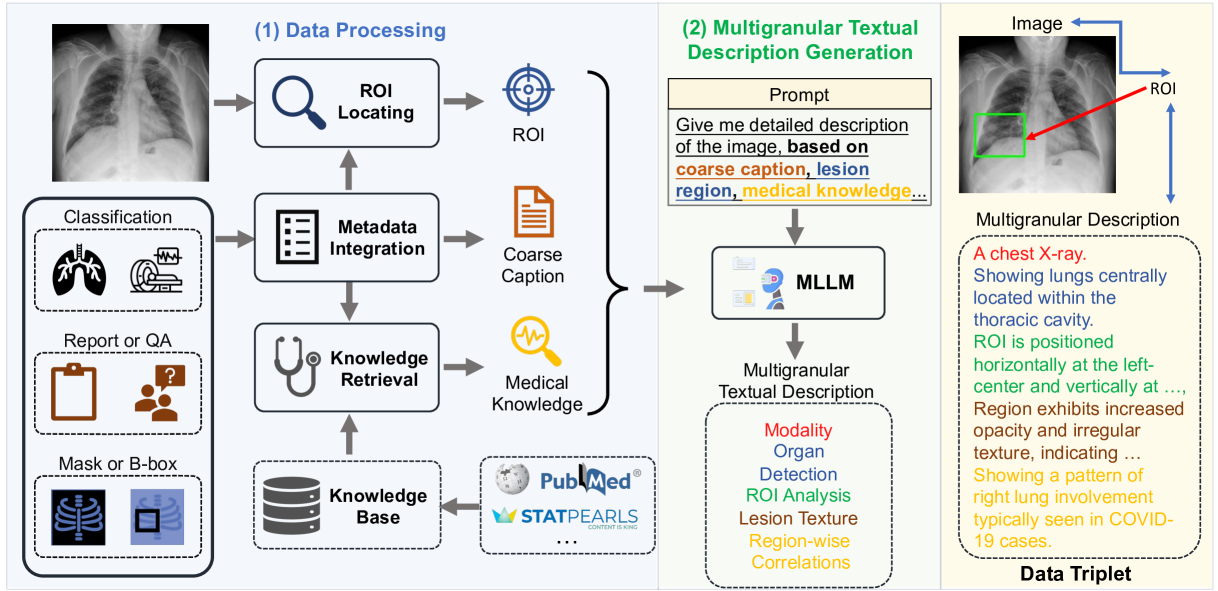
\includegraphics[width=0.95\linewidth]{reading/paper_deep_reading/ideas/figures/medtrinity/x1.png}
  \caption{\textbf{MedTrinity-25M 数据构造 pipeline (论文 Fig.~2)。} 整个流程分两阶段：(1) Data Processing —— 由 metadata integration 生成 coarse caption、由 domain-specific expert 做 ROI locating、由 PubMed / StatPearls 等知识库做 medical knowledge retrieval；(2) Multigranular Textual Description Generation —— 把 coarse caption + ROI + medical knowledge 一起喂给 MLLM，按 ``Modality / Organ / Detection / ROI Analysis / Lesion Texture / Region-wise Correlations'' 6 个粒度生成描述，最终得到 ``image $+$ ROI $+$ multigranular description'' 的 \textbf{data triplet}。右侧示例展示了一张 chest X-ray 的 ROI 框（绿色矩形）以及对应的多粒度文字描述。\textbf{这张图直接对应我 idea 中 ``box $+$ 局部描述 $+$ 关系描述'' 的视觉原语监督信号。}}
  \label{fig:medtrinity-pipeline}
\end{figure}

\paragraph{2.3 自动化 pipeline。}

\begin{enumerate}[leftmargin=1.5em]
  \item Coarse caption（先看图说大致内容）；
  \item ROI locating（domain-specific expert models 找异常 / 病灶区域）；
  \item Medical KB retrieval（结合本体 / 教科书检索）；
  \item MLLM 多粒度生成（基于上面三步合成 triplet）。
\end{enumerate}

\paragraph{2.4 规模与覆盖。}
25M+ 图像，10 模态（CT / MRI / X-ray / 超声 / 病理 / 内镜 / 眼底 / 皮肤镜 / OCT / 显微镜），65+ 疾病，源自 30+ 个公开数据集。

\begin{figure}[H]
  \centering
  \begin{minipage}{0.46\linewidth}
    \centering
    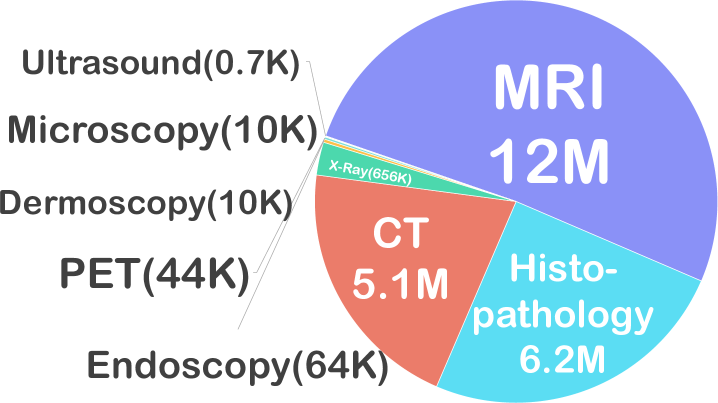
\includegraphics[width=\linewidth]{reading/paper_deep_reading/ideas/figures/medtrinity/x9.png}
    \subcaption{Modality distribution（论文 Fig.~8a）}
  \end{minipage}\hfill
  \begin{minipage}{0.46\linewidth}
    \centering
    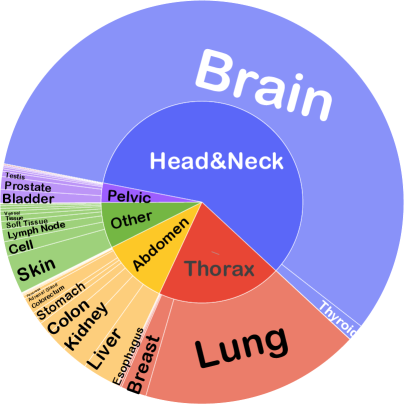
\includegraphics[width=\linewidth]{reading/paper_deep_reading/ideas/figures/medtrinity/x10.png}
    \subcaption{Biological structures（论文 Fig.~8b）}
  \end{minipage}
  \caption{\textbf{MedTrinity-25M 统计概览。} 左：10 大模态的样本占比，可以看到 X-ray / 病理 / CT 占绝对主体——这意味着我做视觉原语 SFT 时不能直接 uniform 采样，否则少数模态（如皮肤镜 / OCT）会被淹没；右：覆盖的解剖结构分布，覆盖了头颈、胸腹、骨骼肌肉、皮肤等大部分器官系统。}
  \label{fig:medtrinity-stats}
\end{figure}

\paragraph{2.5 与既有数据集的定性对比。}
论文 Fig.~1 把 MedTrinity 的 triplet 与两类典型医学多模态资源做了正面对照：(a) 与含放射报告的 MIMIC-CXR 比较，(b) 与 VQA 数据集 SLAKE 比较。结论：MIMIC 的报告偏\textbf{临床印象},缺乏\textbf{空间定位}与\textbf{量化测量}；SLAKE 的 QA 偏\textbf{single-fact}，缺乏\textbf{多粒度的连续描述}。MedTrinity 的 triplet 同时给出 ``box + 多粒度文字 + region-wise relation''，这是我做视觉原语推理唯一直接可用的形态。

\begin{figure}[H]
  \centering
  \begin{minipage}{0.95\linewidth}
    \centering
    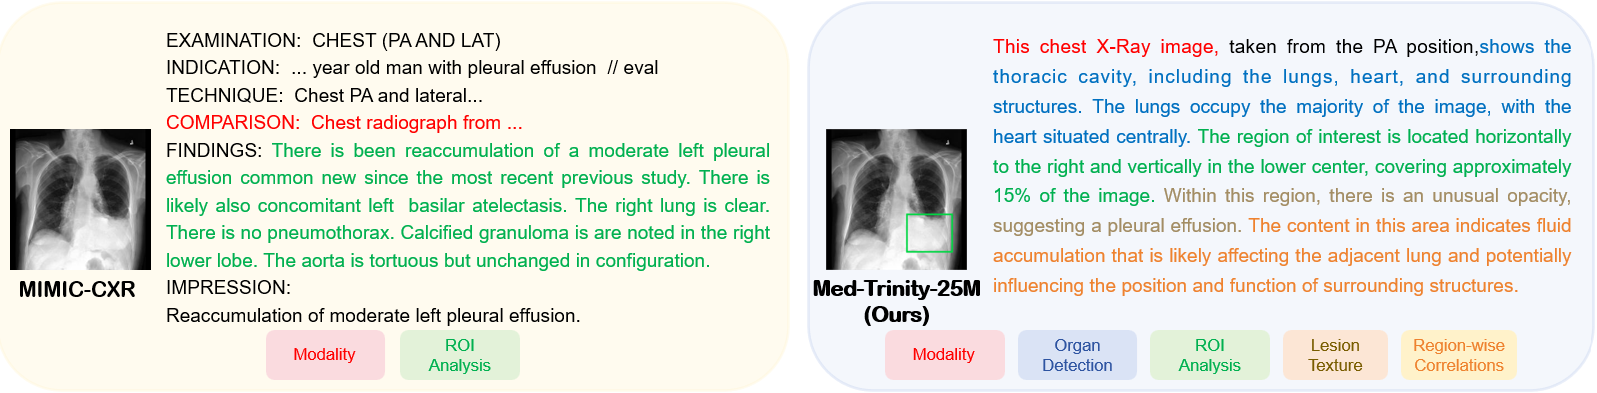
\includegraphics[width=\linewidth]{reading/paper_deep_reading/ideas/figures/medtrinity/compare_mimic.png}
    \subcaption{vs MIMIC-CXR：放射报告侧重临床印象，无显式空间定位（论文 Fig.~1a）}
  \end{minipage}\\[0.6em]
  \begin{minipage}{0.95\linewidth}
    \centering
    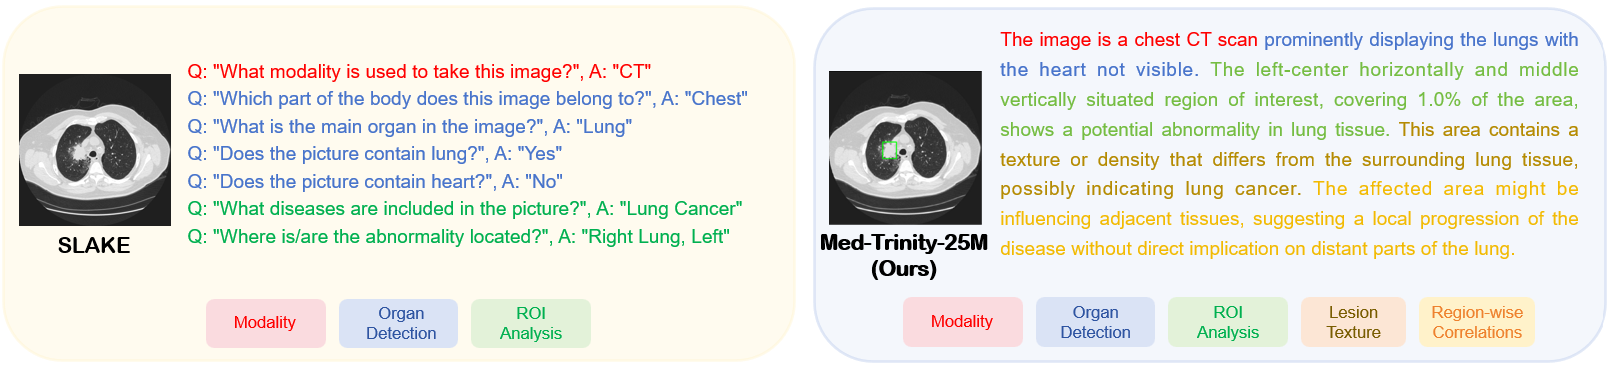
\includegraphics[width=\linewidth]{reading/paper_deep_reading/ideas/figures/medtrinity/compare_slake.png}
    \subcaption{vs SLAKE：VQA 形式回答 single-fact，缺乏多粒度连续描述（论文 Fig.~1b）}
  \end{minipage}
  \caption{\textbf{MedTrinity-25M triplet 相对既有数据形态的优势 (论文 Fig.~1)。} MedTrinity 把 ``空间定位 + 多粒度描述 + 区域关系'' 一次性整合进同一条样本，正好满足 TWVP 范式所需的全部监督粒度。}
  \label{fig:medtrinity-compare}
\end{figure}

\paragraph{2.6 配套模型 LLaVA-Tri。}
在 LLaVA 上用 MedTrinity-25M 预训，VQA-RAD / SLAKE / PathVQA 上拿到 SOTA。

\paragraph{2.7 对我的启示。}

\begin{enumerate}[leftmargin=1.5em]
  \item \textbf{这是 idea 的主数据}：``triplet 单元'' 几乎完美匹配 TWVP 的 ``box + 局部 desc + 关系 desc''；
  \item \textbf{自动 pipeline 思想可复用}：当我要把 idea 扩到没有 GT bbox 的子领域（如 Lingshu 训练数据里的 ROCOv2 / PMC-VQA），可以用 ``MLLM-pseudo-bbox + 一致性过滤'' 自己造监督信号；
  \item \textbf{风险点}：由于是 LLM 合成，需注意 ``幻觉描述''——我可以把 MedReason 的 KG-validate 思路套上去做二次过滤。
\end{enumerate}

\subsubsection*{3. GMAI-VL \& GMAI-VL-5.5M (CVPR 2025 / arXiv 2411.14522)}

\textbf{作者：} Tianbin Li 等 (Shanghai AI Lab + 多校)。\\
\textbf{核心一句话：} 这篇不是单纯提出一个模型，而是同时给出一个 \textbf{5.5M 级通用医学多模态数据集 GMAI-VL-5.5M} 和一个基于该数据训练的 \textbf{general medical LVLM：GMAI-VL}。对我的项目来说，它最重要的价值不是 benchmark 分数，而是它把多源医学图像数据统一成了可训练的 annotation-guided instruction 数据，其中的 bbox-level caption 正好能作为视觉原语 SFT 的补充来源。

\paragraph{3.1 总览：数据、模型、训练 recipe 被放在同一张图里。}

\begin{figure}[H]
  \centering
  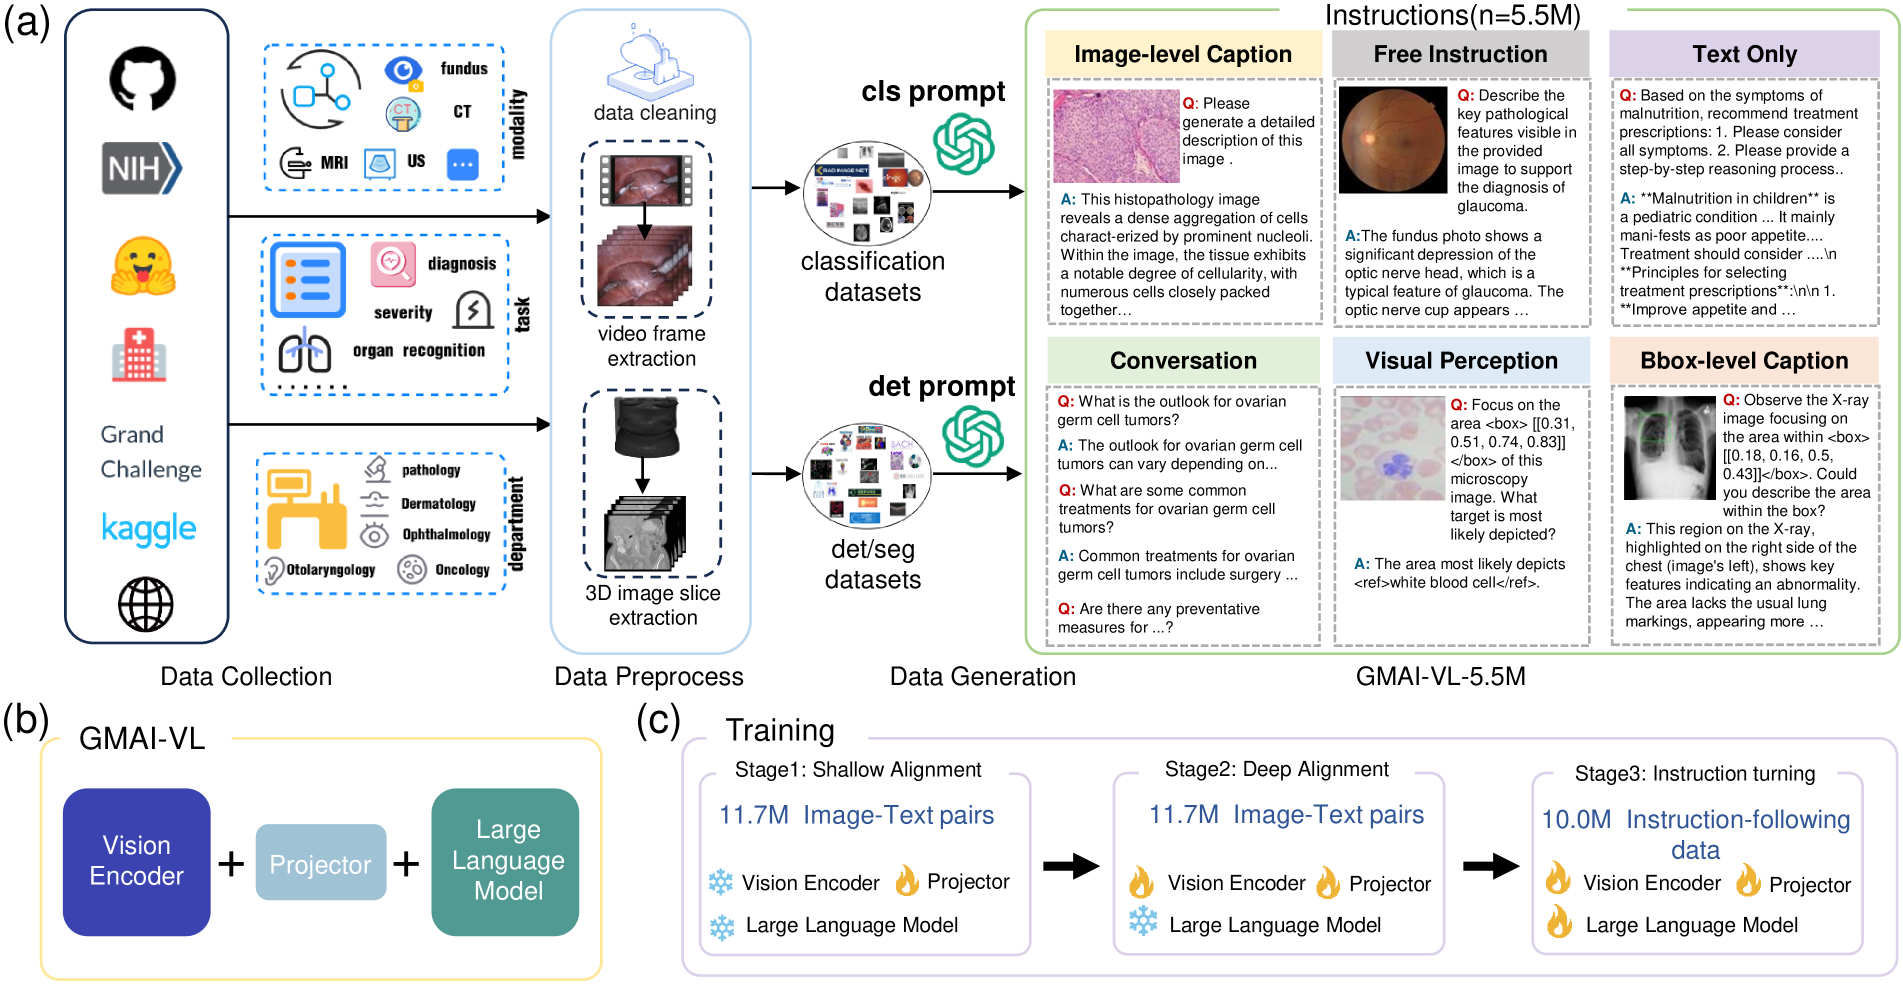
\includegraphics[width=0.98\linewidth]{reading/paper_deep_reading/ideas/figures/gmai_vl/x1.png}
  \caption{\textbf{GMAI-VL 与 GMAI-VL-5.5M 总览（论文 Fig.~1）。} (a) GMAI-VL-5.5M 的数据构造：从 GitHub / NIH / HuggingFace / Grand Challenge / Kaggle / 网页等来源收集医学数据，按 modality、task、department 做清洗和标准化；视频抽帧、3D 图像切片后，通过 classification prompt 和 detection/segmentation prompt 转换成 image-level caption、free instruction、text-only、conversation、visual perception、bbox-level caption 等多种 instruction 格式。(b) GMAI-VL 模型结构仍是典型 LVLM 三件套：Vision Encoder $+$ Projector $+$ LLM。(c) 训练 recipe 分三阶段：shallow alignment、deep alignment、instruction tuning。\textbf{对我的启发：} 这张图说明 GMAI-VL 的关键不在结构创新，而在 ``多源标注 $\to$ instruction 数据'' 的工程化统一；这正是我把医学视觉原语接入 Lingshu / Qwen2.5-VL 时最需要复用的部分。}
  \label{fig:gmai-vl-overview}
\end{figure}

\paragraph{3.2 数据集贡献。}
GMAI-VL-5.5M 把 \textbf{219 个专科医学数据集} 转换成统一的 high-quality image-text pairs，整体规模为 5.5M，覆盖 13 种医学模态与 18 个临床专科。论文强调三点：
\begin{itemize}[leftmargin=1.5em]
  \item \textbf{Comprehensive medical tasks}：覆盖疾病类型、症状、治疗、诊疗流程等多种任务，不只是单一 VQA；
  \item \textbf{Rich multimodal representation}：包含 CT、MRI、X-ray、超声、内镜、病理、眼底等多模态图像，也包含报告、病历等文本；
  \item \textbf{Annotation-guided generation}：不是让 GPT 对图像自由发挥，而是把可信数据集里的 modality、task type、label、bbox 等结构化标注转成 prompt，降低幻觉风险。
\end{itemize}

\begin{figure}[H]
  \centering
  \begin{minipage}{0.48\linewidth}
    \centering
    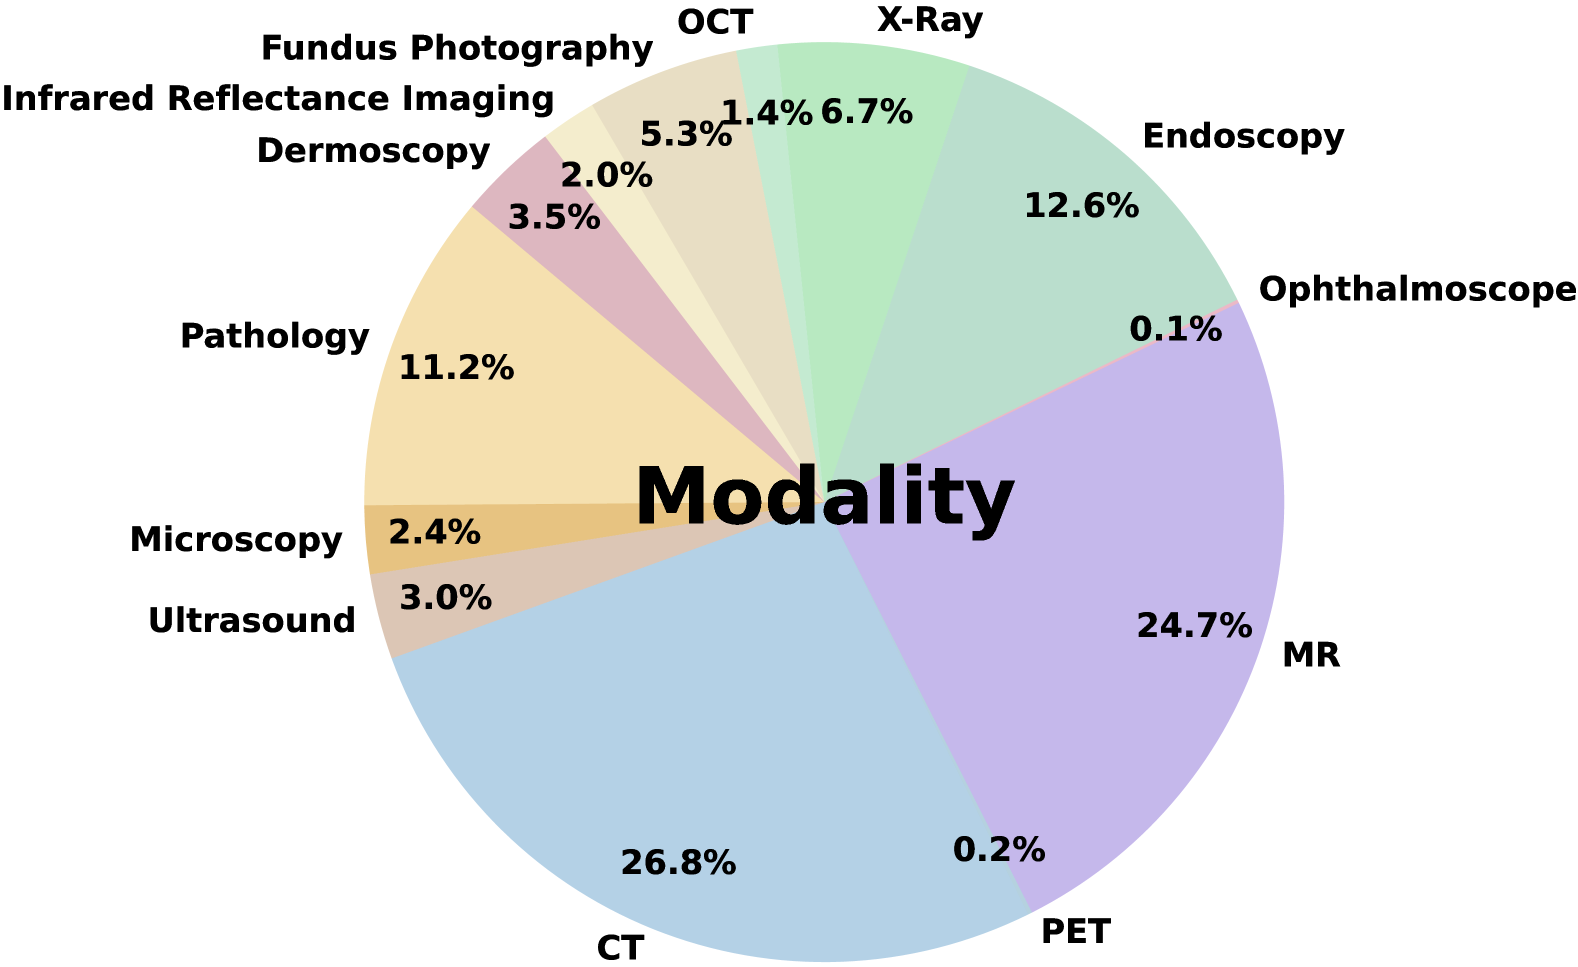
\includegraphics[width=\linewidth]{reading/paper_deep_reading/ideas/figures/gmai_vl/x7.png}
    \subcaption{Modality distribution}
  \end{minipage}\hfill
  \begin{minipage}{0.48\linewidth}
    \centering
    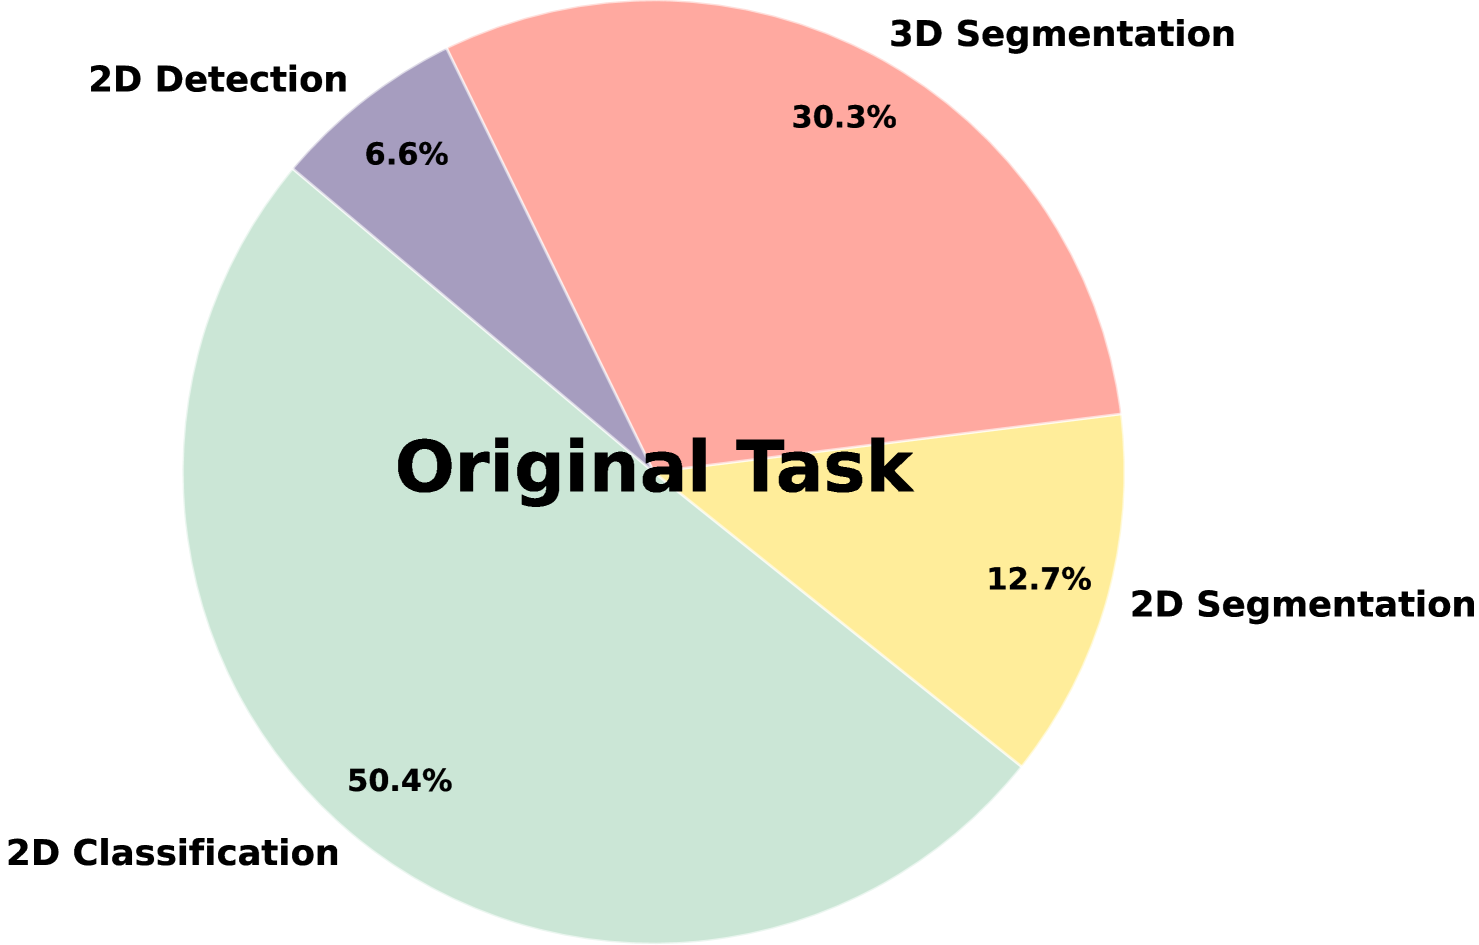
\includegraphics[width=\linewidth]{reading/paper_deep_reading/ideas/figures/gmai_vl/x8.png}
    \subcaption{Original task distribution}
  \end{minipage}\\[0.6em]
  \begin{minipage}{0.48\linewidth}
    \centering
    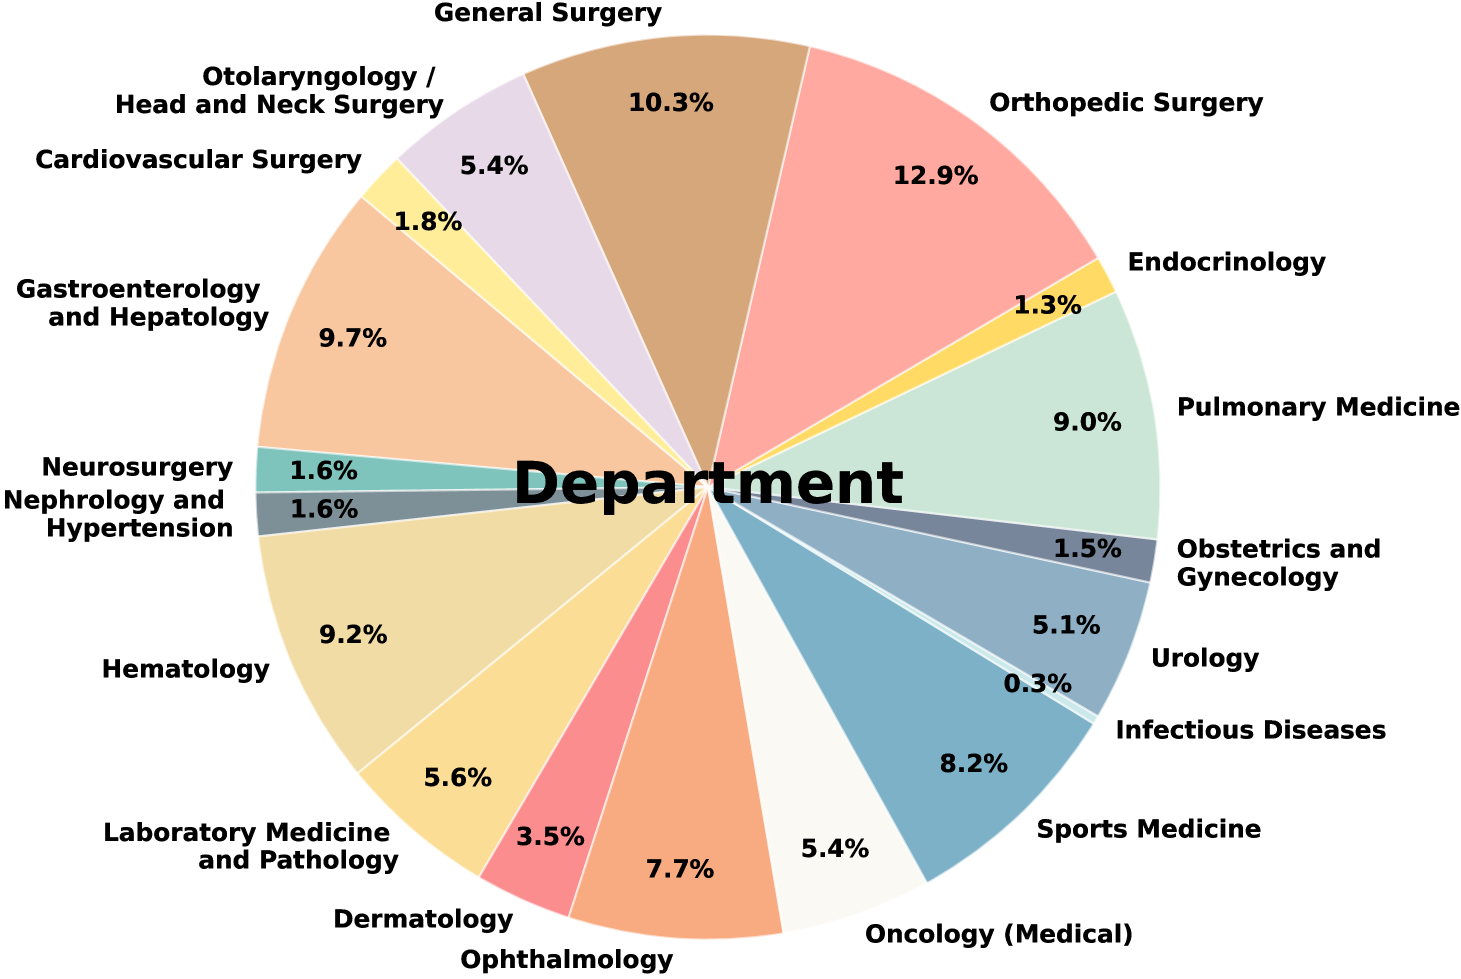
\includegraphics[width=\linewidth]{reading/paper_deep_reading/ideas/figures/gmai_vl/x9.png}
    \subcaption{Department distribution}
  \end{minipage}\hfill
  \begin{minipage}{0.48\linewidth}
    \centering
    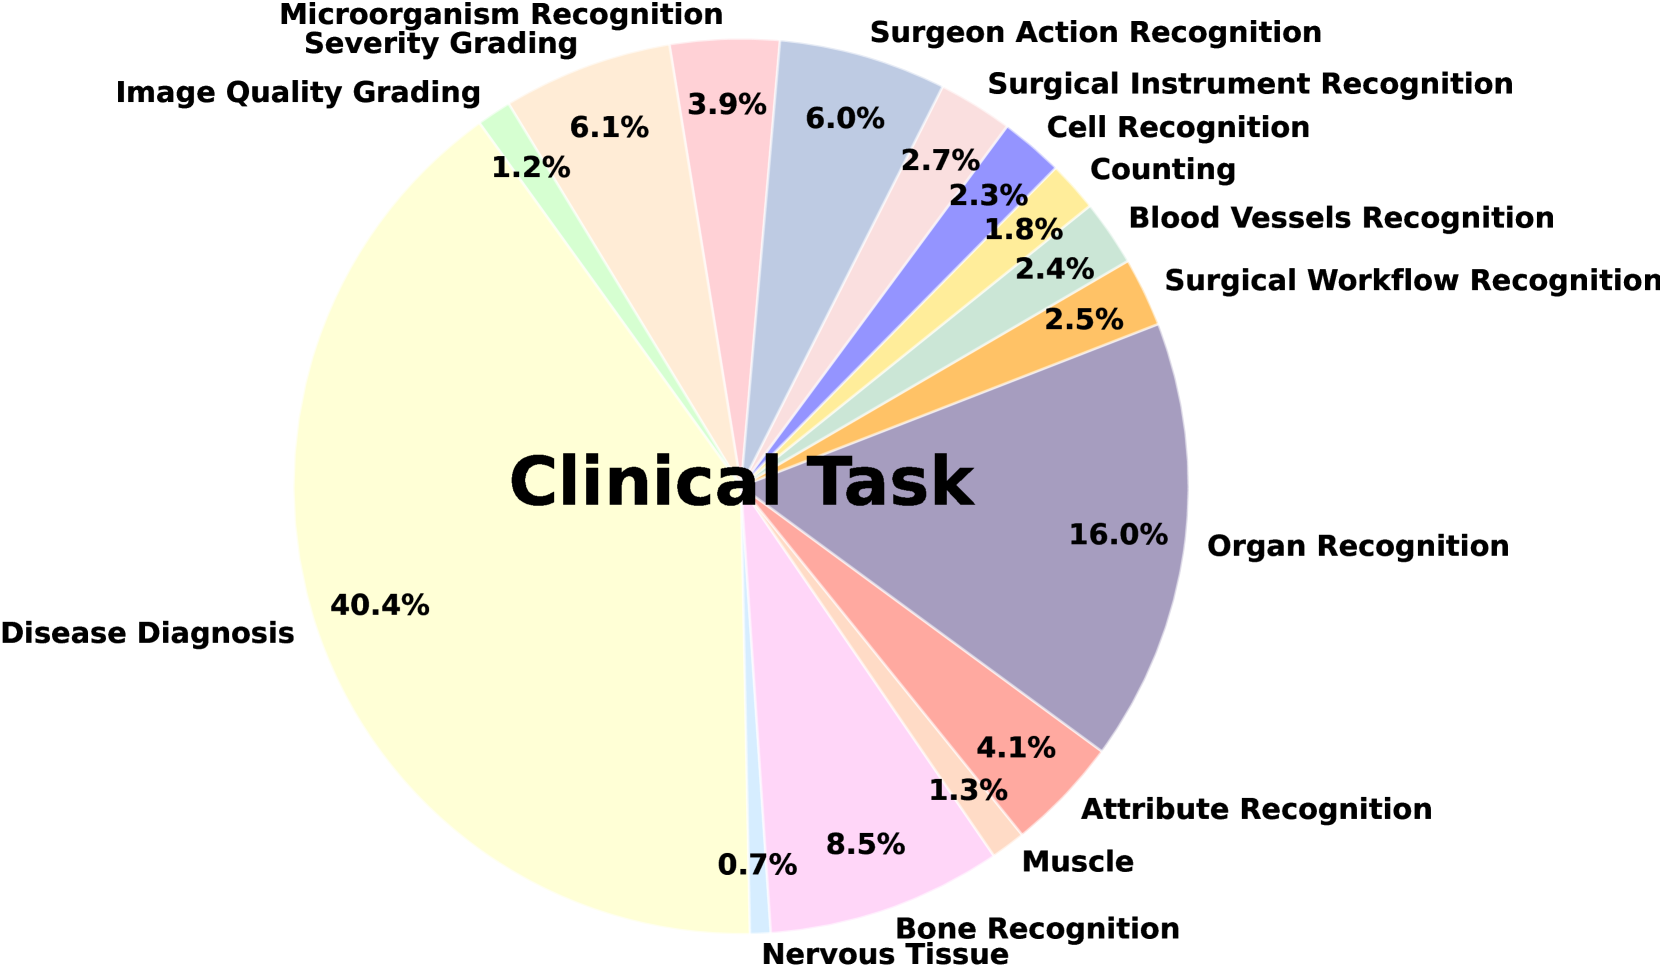
\includegraphics[width=\linewidth]{reading/paper_deep_reading/ideas/figures/gmai_vl/x10.png}
    \subcaption{Clinical task distribution}
  \end{minipage}
  \caption{\textbf{GMAI-VL-5.5M 的数据分布（补充材料 Fig.~3）。} 四张图分别展示模态、原始任务、临床科室与临床任务分布。结合论文 Table~3：任务类型中 2D classification 占 50.4\%，3D segmentation 占 30.3\%，2D segmentation 占 12.7\%，2D detection 占 6.6\%；模态中 CT 占 26.8\%，MR 占 24.7\%，Endoscopy 占 12.6\%，Pathology 占 11.2\%，X-ray 占 6.7\%，Fundus 占 5.3\%，Ultrasound 占 3.0\%。\textbf{这意味着：} 如果我直接拿 GMAI-VL-5.5M 做视觉原语 SFT，需要做 modality-balanced / task-balanced sampling，否则模型会被 CT/MR 和 classification/segmentation 主导。}
  \label{fig:gmai-vl-5m-distribution}
\end{figure}

\paragraph{3.3 关键技术——空间标注的统一化。}

\begin{itemize}[leftmargin=1.5em]
  \item 把 \textbf{SA-Med2D-20M 的 segmentation mask 转成 detection bbox}（mask 取外接矩形），这是视觉原语监督的关键金矿；
  \item 标注 schema 统一为 $\langle$image, modality, label, department, bbox [optional]$\rangle$；
  \item \textbf{对话样例}：``As a medical expert, you are given a $\langle$X-ray$\rangle$ image \dots where the $\langle$bbox [179,164,500,434]$\rangle$ is labeled as $\langle$Pneumothorax$\rangle$''；
  \item 生成策略是 \textbf{annotation-guided prompt}：classification 数据走 cls prompt，detection / segmentation 数据走 det prompt；最终统一成 caption、conversation、visual perception、bbox-level caption 等 instruction 格式。
\end{itemize}

\paragraph{3.4 训练数据与模型 recipe。}

\begin{figure}[H]
  \centering
  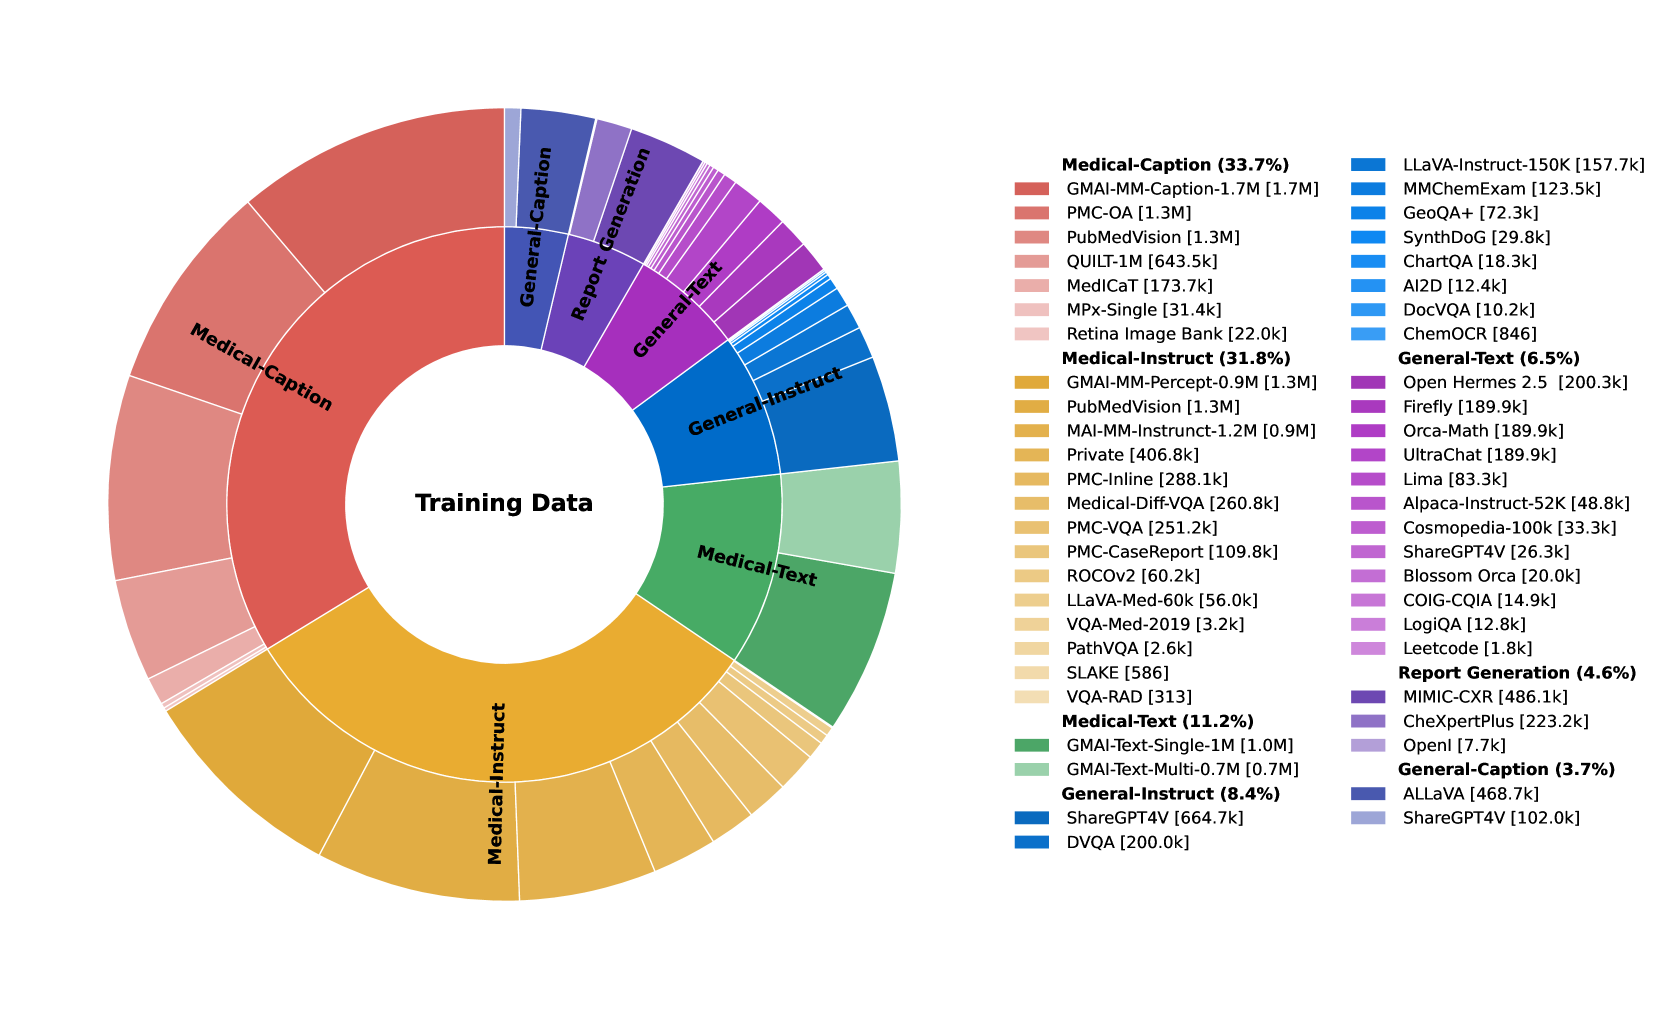
\includegraphics[width=0.74\linewidth]{reading/paper_deep_reading/ideas/figures/gmai_vl/x11.png}
  \caption{\textbf{GMAI-VL 训练数据分布（补充材料 Fig.~4）。} 内环表示训练数据的大类，外环表示对应子类，扇区大小与数据量成比例。结合 Fig.~1(c)，GMAI-VL 采用三阶段训练：Stage 1 shallow alignment 使用 11.7M image-text pairs，冻结 vision encoder 与 LLM，仅训练 projector；Stage 2 deep alignment 继续使用 11.7M image-text pairs，同时训练 vision encoder 与 projector、冻结 LLM；Stage 3 instruction tuning 使用 10.0M instruction-following data，同时训练 vision encoder、projector 和 LLM。\textbf{对我的启发：} 如果我的目标是提升 Lingshu 的视觉原语推理能力，不一定要重训完整 LVLM；更现实的 recipe 是先做一个轻量 visual-primitive SFT / adapter alignment，再接 RLVR。}
  \label{fig:gmai-vl-training-data}
\end{figure}

\paragraph{3.5 模型 GMAI-VL 与结果案例。}
GMAI-VL 的架构没有复杂化：Vision Encoder 负责视觉特征，Projector 把视觉 token 映射到 LLM 空间，LLM 负责医学语言理解与生成。论文真正的贡献是：用大规模医学 image-text 数据完成视觉-语言对齐，再用 instruction-following 数据注入诊断、定位、描述、对话等任务能力。

\begin{figure}[H]
  \centering
  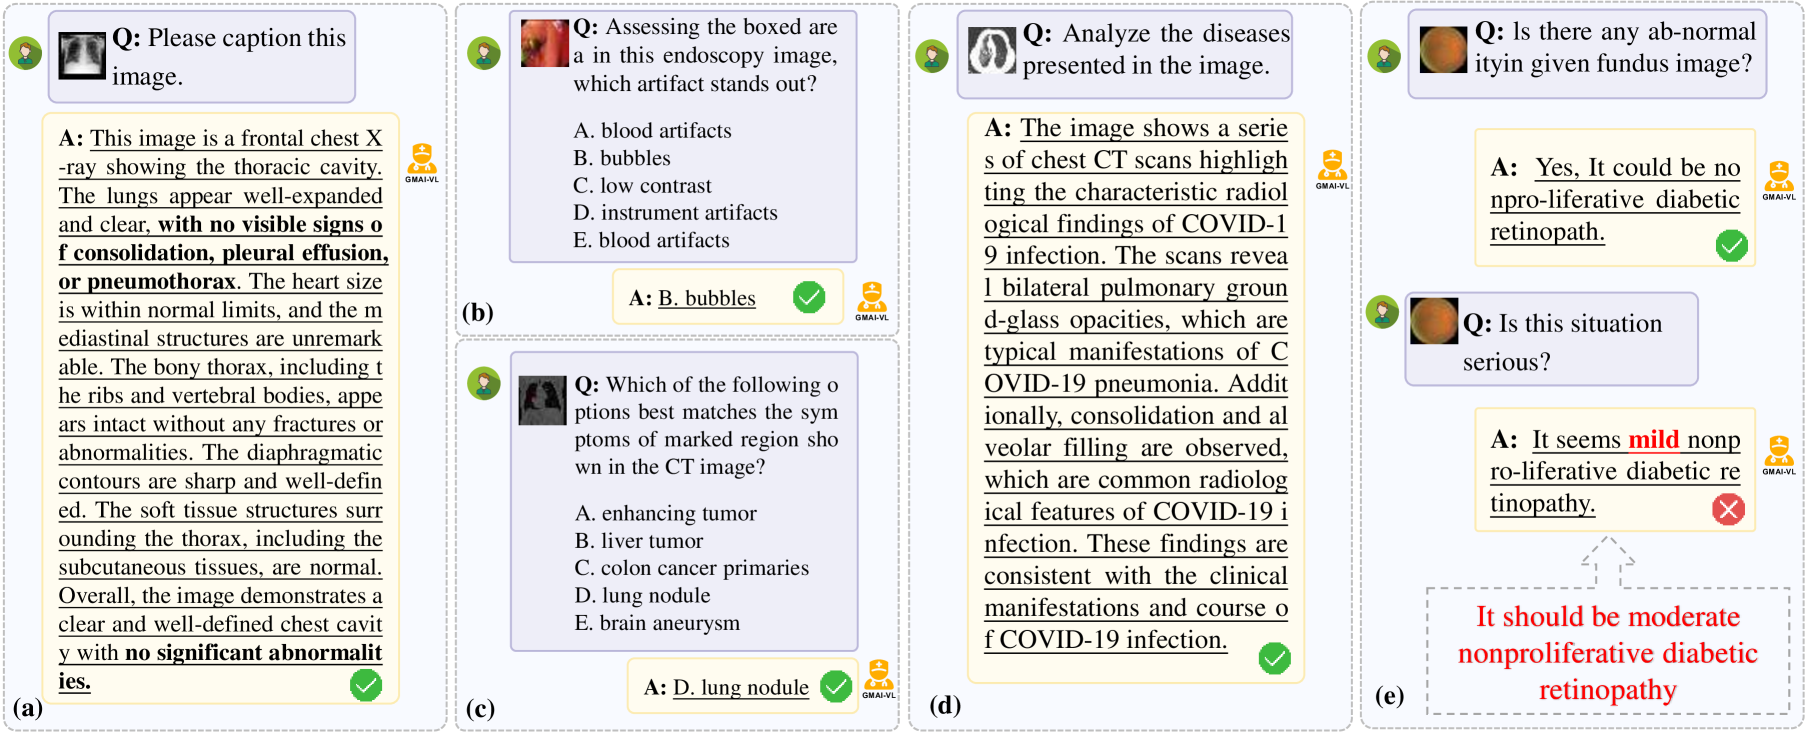
\includegraphics[width=0.98\linewidth]{reading/paper_deep_reading/ideas/figures/gmai_vl/x6.png}
  \caption{\textbf{GMAI-VL 输出案例（论文 Fig.~2）。} 图中展示了 image caption、bbox 区域识别、多选诊断、疾病分析、眼底病变判断等任务。前四个例子说明模型能生成较完整的医学描述，并能利用 boxed area 做局部判断；(e) 是失败案例：模型把 moderate nonproliferative diabetic retinopathy 误判成 mild。\textbf{这对我的启发很关键：} 即使经过大规模医学 instruction tuning，模型仍可能在 severity grading / fine-grained diagnosis 上失败；因此我的 ``视觉原语后训练'' 不应只奖励最终答案，还应奖励中间过程是否正确定位病灶、是否描述了关键局部征象、是否把局部征象与诊断等级关联起来。}
  \label{fig:gmai-vl-examples}
\end{figure}

\paragraph{3.6 对我的启示。}

\begin{enumerate}[leftmargin=1.5em]
  \item \textbf{Prompt 模板可直接复用}：TWVP 的 \texttt{<|ref|>...<|/ref|><|box|>...<|/box|>} 格式可以无缝对接 GMAI-VL 的 bbox-level caption / visual perception 样例；
  \item \textbf{GMAI-VL-5.5M 是 MedTrinity-25M 的补充而不是替代}：MedTrinity 更强调 image-ROI-description triplet 和 region-wise relation；GMAI-VL-5.5M 更强调多源数据统一、任务多样性与 bbox-level instruction；两者合起来能覆盖 ``定位 $+$ 描述 $+$ 问答 $+$ 临床任务''；
  \item \textbf{mask $\to$ bbox 这一步可以直接复用}：GMAI-VL 已经把 SA-Med2D-20M 的 mask 外接矩形化，省掉大量预处理；如果后续做 ``thinking with masks''，还可以反向回到原始 mask；
  \item \textbf{训练策略提醒我不要只做 SFT}：Fig.~2 的失败案例说明，大规模 SFT 后模型仍会在细粒度病情分级上出错；更合理的路线是先用 bbox / mask / ROI description 做视觉原语 SFT，再用可验证任务做 RL，把 reward 设计成 answer accuracy + format + localization / evidence consistency。
\end{enumerate}

\subsubsection*{4. VILA-M3 (CVPR 2025 / arXiv 2411.12915)}

\textbf{作者：} Vishwesh Nath 等，NVIDIA + MONAI 团队。\\
\textbf{论文来源：} \href{https://arxiv.org/abs/2411.12915}{arXiv 2411.12915} / \href{https://arxiv.org/html/2411.12915v3}{HTML v3} / \href{https://github.com/Project-MONAI/VLM}{Project-MONAI/VLM}。\\
\textbf{核心一句话：} VILA-M3 的关键不是发明新的 VLM 架构，而是把医疗领域已经很强的 narrow expert models（BraTS、VISTA3D、TorchXRayVision 等）接进 VLM 的 instruction tuning 和推理链路：VLM 负责理解用户意图、选择专家模型与参数，专家模型负责提供细粒度 segmentation / classification 证据，最后 VLM 再基于这些证据生成医学回答。

\paragraph{4.1 核心思想——第四阶段 specialized IFT + 专家模型反馈。}
作者认为通用 VLM（GPT-4o / Gemini）在医学上不够，因为它们主要依赖互联网知识和粗粒度视觉-语言对齐，缺乏医疗专家模型学到的细粒度影像特征。传统 VILA/VLM 通常有三阶段训练：projector pre-training、vision-language pre-training、instruction fine-tuning；VILA-M3 在此基础上加入 \textbf{Step 3: Expert Information Guided Instruction Fine-Tuning}，也就是把专家模型卡片、专家调用格式和专家输出反馈纳入 IFT。

\begin{figure}[H]
  \centering
  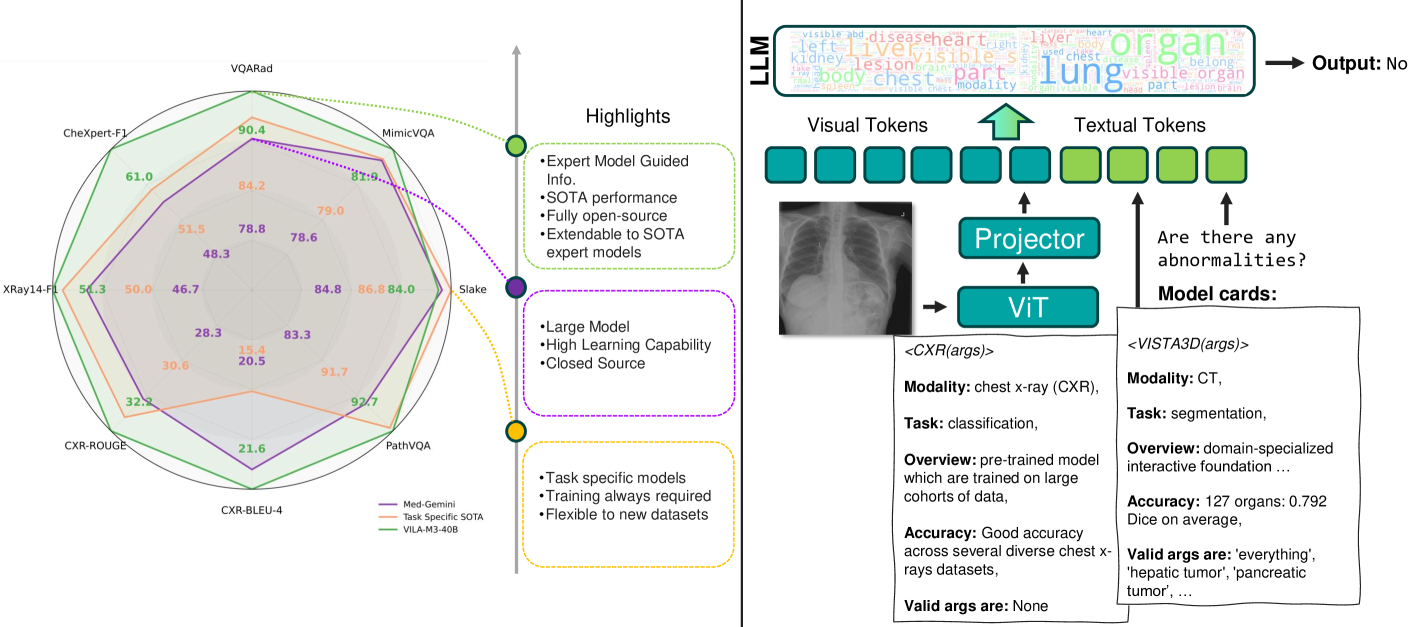
\includegraphics[width=0.98\linewidth]{reading/paper_deep_reading/ideas/figures/vila_m3/x1.png}
  \caption{\textbf{VILA-M3 总览（论文 Fig.~1）。} 左侧雷达图比较 VILA-M3-40B、Med-Gemini 与任务专用 SOTA，论文报告 VILA-M3 平均比 Med-Gemini 提升约 9\%，比任务专用模型提升约 6\%。右侧是架构示意：图像经 ViT 与 projector 变成 visual tokens，用户 prompt 作为 textual tokens，同时系统提示中提供 expert model cards，例如 \texttt{<CXR(args)>} 与 \texttt{<VISTA3D(args)>}，包括 modality、task、overview、accuracy、valid args 等信息。\textbf{对我的启发：} 这相当于把 ``可调用医学视觉原语工具库'' 放进模型上下文，让模型学习什么时候调用、调用哪个工具、传什么参数。}
  \label{fig:vila-m3-overview}
\end{figure}

\paragraph{4.2 训练框架：从通用 VILA 到医学专家引导 IFT。}
VILA-M3 选择 VILA 作为底座，因为 VILA 是 auto-regressive multimodal LLM：图像被 tokenized 成 visual tokens，与 text tokens 拼接后输入 LLM；projector 负责把 vision encoder 的 embedding 映射到语言模型空间。论文沿用 VILA 的基本训练流程，但在最后增加 expert-guided IFT：
\begin{enumerate}[leftmargin=1.5em]
  \item \textbf{Step 0 Projector Pre-training}：冻结 LLM 与 vision encoder，只训练 projector，让模型适配 image tokens；
  \item \textbf{Step 1 Vision-Language Pre-training}：学习视觉和语言 embedding 的对应关系；
  \item \textbf{Step 2 Instruction Fine-Tuning}：增强语言对话能力和输出连贯性；
  \item \textbf{Step 3 Expert Information Guided IFT}：加入医疗 instruction tuning data 与 expert model guidance，让模型学会把专家模型作为外部知识源使用。
\end{enumerate}

\begin{figure}[H]
  \centering
  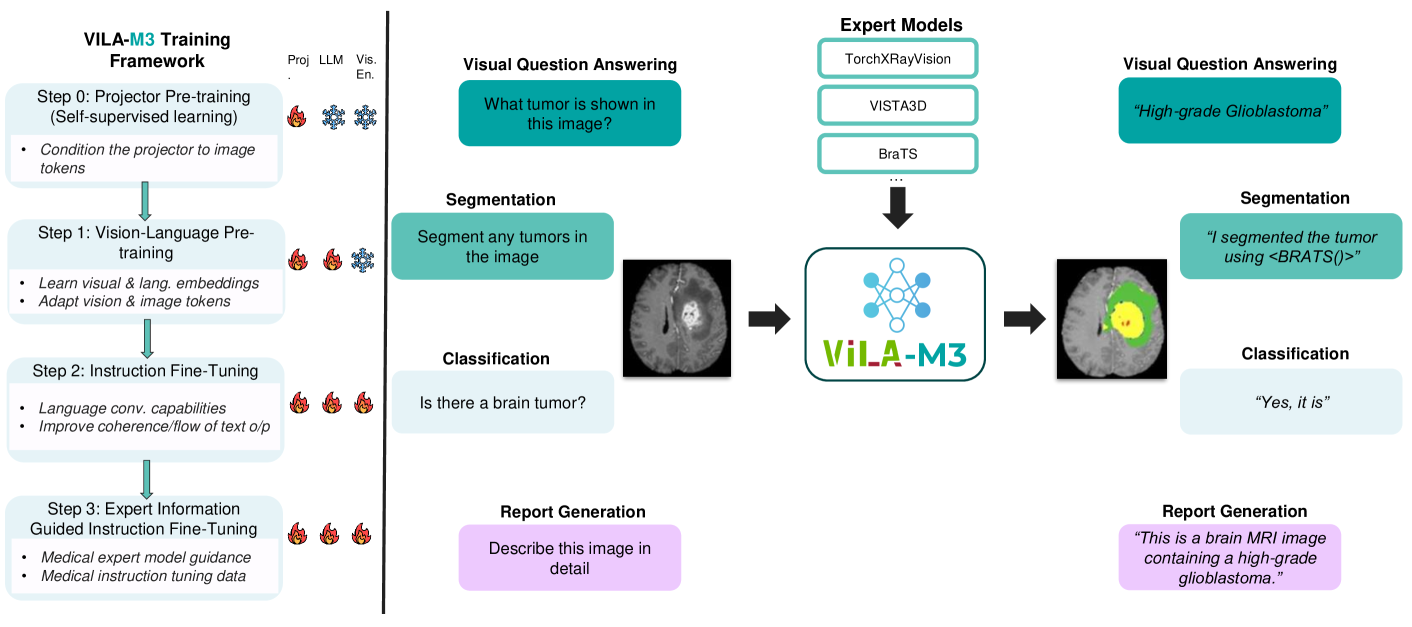
\includegraphics[width=0.98\linewidth]{reading/paper_deep_reading/ideas/figures/vila_m3/x2.png}
  \caption{\textbf{VILA-M3 训练框架与多任务能力（论文 Fig.~2）。} 左侧展示四步训练流程；右侧展示 VQA、segmentation、classification、report generation 等任务。对于 segmentation，VILA-M3 不一定自己直接画 mask，而是选择合适专家模型，例如用 BraTS 完成脑肿瘤分割，再把 expert 输出作为证据用于回答。\textbf{关键点：} VILA-M3 把 ``医学专家模型'' 从离线数据生成器提升成了模型可按需触发的推理组件。}
  \label{fig:vila-m3-framework}
\end{figure}

\paragraph{4.3 推理时挂载专家：keyword + argument 的工具调用。}
推理时，VLM 通过 special token / tool-call 形式调用外部 expert。例如论文给出的格式是 \texttt{<VISTA3D(hepatic tumor)>}：
\begin{itemize}[leftmargin=1.5em]
  \item \textbf{BraTS}：脑肿瘤 segmentation；
  \item \textbf{VISTA3D}：全身 CT/3D anatomy 与 lesion segmentation，可传入 \texttt{hepatic tumor}、\texttt{skeleton}、\texttt{everything} 等参数；
  \item \textbf{TorchXRayVision / CXR expert}：胸片分类；
  \item 其他 expert 以 model card 方式暴露给 VLM，模型根据用户任务选择专家与参数。
\end{itemize}
专家输出 mask / class / overlay 后，重新作为视觉或文本上下文喂回 VLM，使模型能基于专家证据生成回答。

\begin{figure}[H]
  \centering
  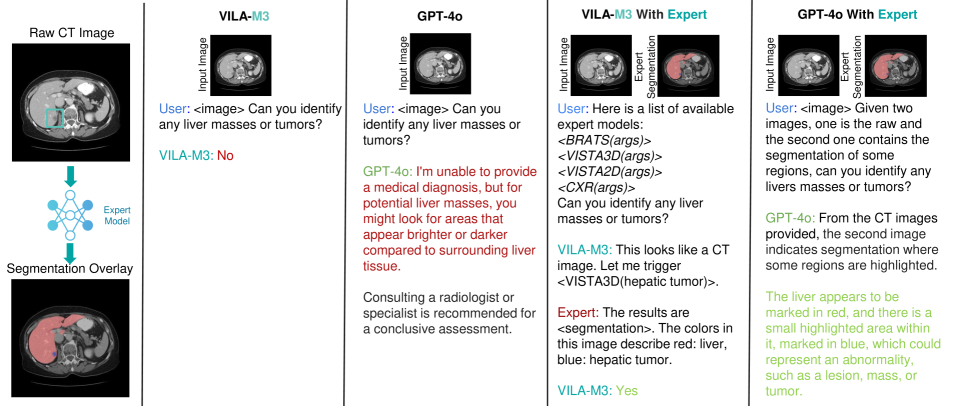
\includegraphics[width=0.88\linewidth]{reading/paper_deep_reading/ideas/figures/vila_m3/x3.png}
  \caption{\textbf{专家分割反馈改善 VLM 诊断质量（论文 Fig.~3）。} 原始 CT 中肝脏肿瘤是细粒度局部征象。没有 expert segmentation 时，VILA-M3 直接回答 ``No''，GPT-4o 也只能给出不确定提示；加入专家分割 overlay 后，VILA-M3 触发 \texttt{<VISTA3D(hepatic tumor)>}，专家返回 liver 与 hepatic tumor 区域，模型最终能回答存在肿瘤。\textbf{这张图直接支持我的核心假设：} 医学 VLM 的失败往往不是语言推理不够，而是缺少可靠的局部视觉证据；bbox/mask/ROI 视觉原语可以作为 evidence bridge。}
  \label{fig:vila-m3-expert-feedback}
\end{figure}

\begin{figure}[H]
  \centering
  \begin{minipage}{0.24\linewidth}
    \centering
    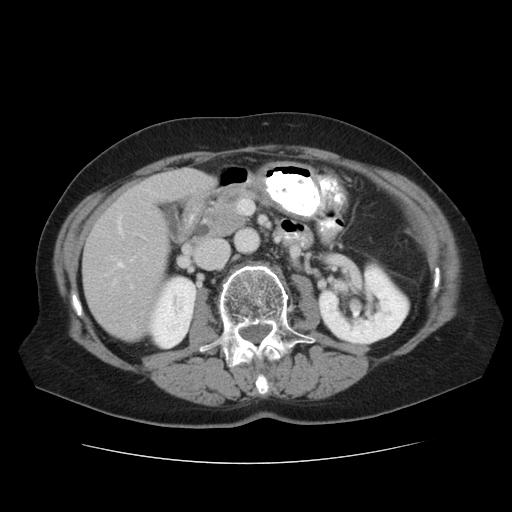
\includegraphics[width=\linewidth]{reading/paper_deep_reading/ideas/figures/vila_m3/ct_original_slice51.jpg}
    \subcaption{original image}
  \end{minipage}\hfill
  \begin{minipage}{0.24\linewidth}
    \centering
    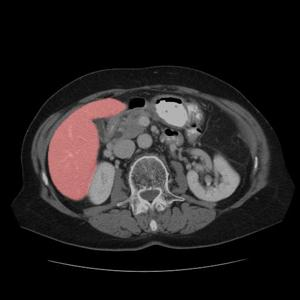
\includegraphics[width=\linewidth]{reading/paper_deep_reading/ideas/figures/vila_m3/ct_liver.jpeg}
    \subcaption{\texttt{hepatic tumor}}
  \end{minipage}\hfill
  \begin{minipage}{0.24\linewidth}
    \centering
    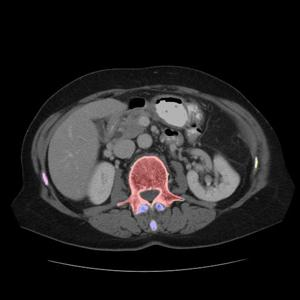
\includegraphics[width=\linewidth]{reading/paper_deep_reading/ideas/figures/vila_m3/ct_bones.jpeg}
    \subcaption{\texttt{skeleton}}
  \end{minipage}\hfill
  \begin{minipage}{0.24\linewidth}
    \centering
    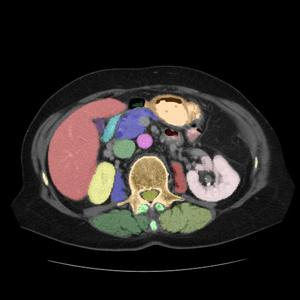
\includegraphics[width=\linewidth]{reading/paper_deep_reading/ideas/figures/vila_m3/ct_everything.jpeg}
    \subcaption{\texttt{everything}}
  \end{minipage}
  \caption{\textbf{VISTA3D 参数选择示例（论文 Fig.~7）。} 同一张 CT slice，VILA-M3 需要根据用户指令选择不同参数：\texttt{hepatic tumor} 对应肝肿瘤，\texttt{skeleton} 对应骨结构，\texttt{everything} 对应全图分割。\textbf{对我的启发：} 工具调用不是简单 ``是否调用分割器''，而是要学习医学语义到视觉原语参数的映射；我的视觉原语 SFT 可以显式构造 \texttt{<|tool|>segment(organ=..., lesion=...)<|/tool|>} 类样本。}
  \label{fig:vila-m3-vista3d-args}
\end{figure}

\paragraph{4.4 实验结论：专家引导有用，但数据平衡和训练轮数很关键。}
论文给出三类对我有用的实验观察：
\begin{itemize}[leftmargin=1.5em]
  \item \textbf{Expert-guided IFT 有效}：VILA-M3 在 VQA、报告生成、分类等任务上超过 Med-Gemini 和任务专用 SOTA；同时在通用 VILA benchmark 上没有严重退化，说明 expert-guided IFT 不是简单过拟合医学任务；
  \item \textbf{专家信息对细粒度诊断尤其关键}：Fig.~3 显示没有 segmentation 时模型漏检肿瘤，有专家 overlay 后才能识别局部病灶；
  \item \textbf{balanced dataset 很重要}：论文把 VQA、expert、report generation、classification 等类别做 frequency balancing，平均带来约 4\% 的指标提升；过多 epoch 会导致性能下降，Fig.~4/Fig.~11 显示 3 epoch 模型出现退化。
\end{itemize}

\begin{figure}[H]
  \centering
  \begin{minipage}{0.48\linewidth}
    \centering
    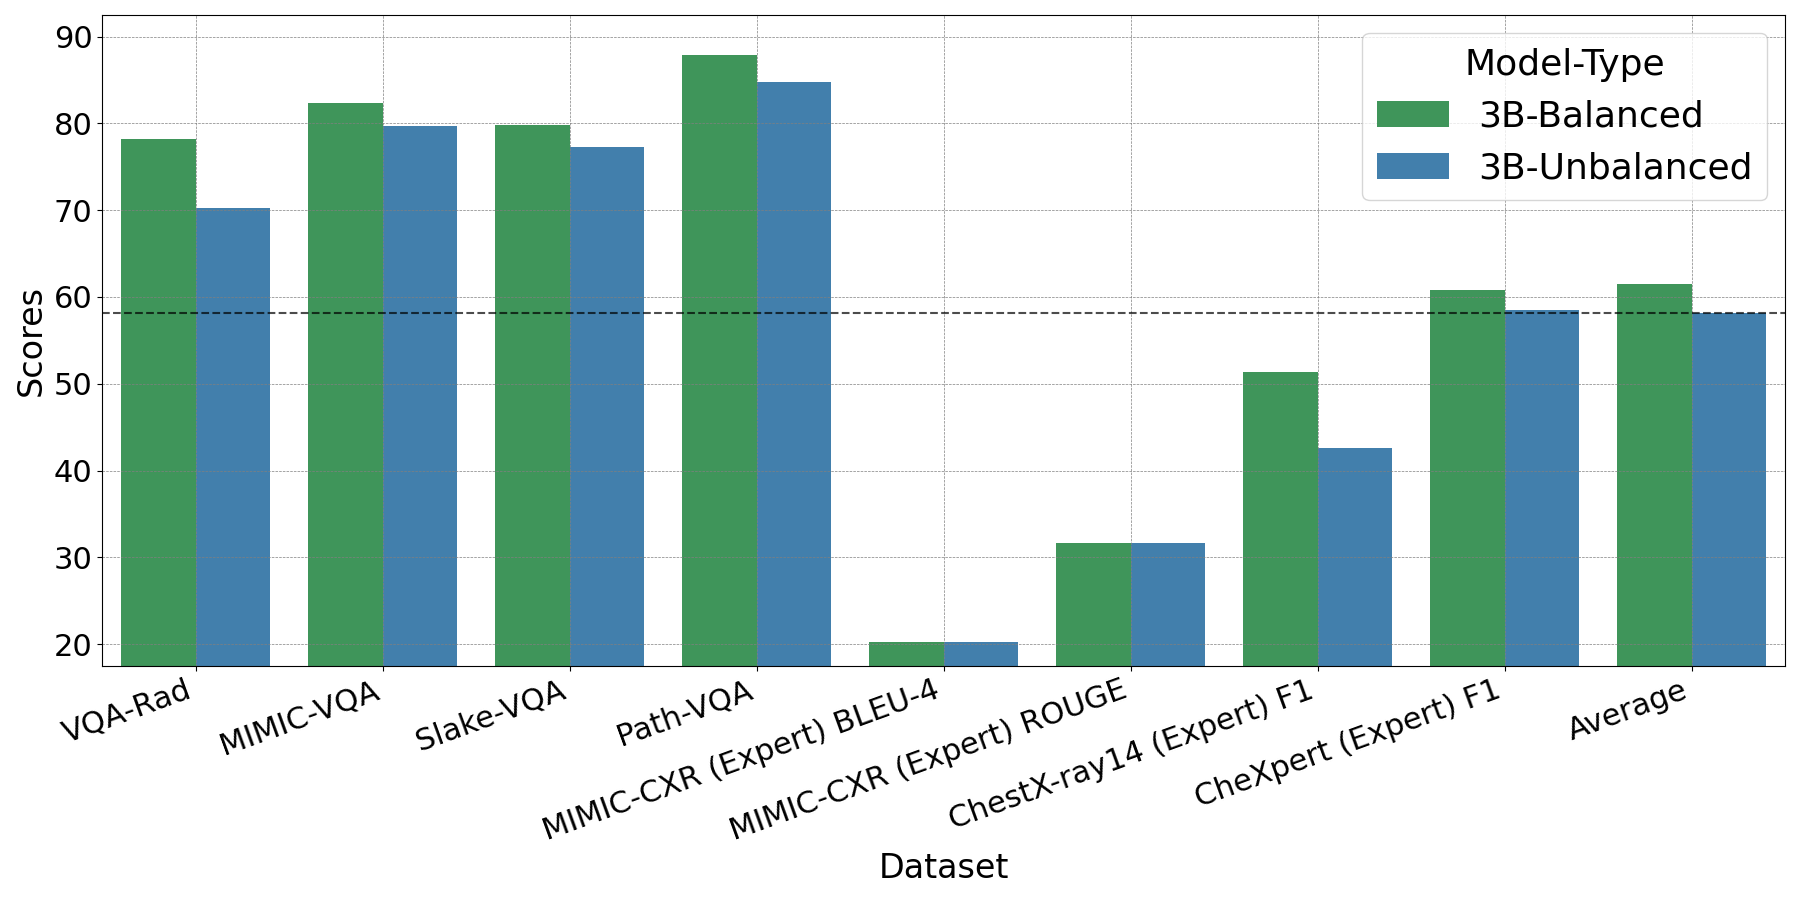
\includegraphics[width=\linewidth]{reading/paper_deep_reading/ideas/figures/vila_m3/fig_9_unba.png}
    \subcaption{Balanced vs. unbalanced healthcare datasets}
  \end{minipage}\hfill
  \begin{minipage}{0.48\linewidth}
    \centering
    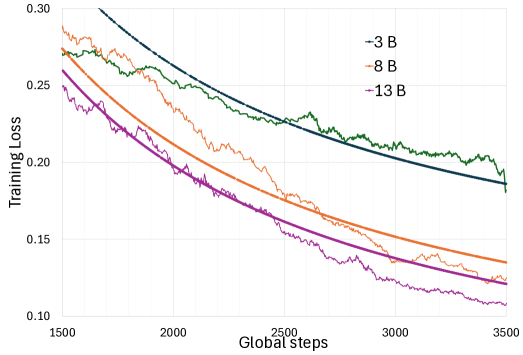
\includegraphics[width=\linewidth]{reading/paper_deep_reading/ideas/figures/vila_m3/x4.png}
    \subcaption{Training loss across model sizes}
  \end{minipage}
  \caption{\textbf{训练稳定性与数据平衡（论文 Fig.~5 / Fig.~6）。} 左图说明 balanced dataset 通常优于直接按原始数据量训练；右图说明不同规模模型的训练 loss 都能正常收敛。\textbf{对我的实验设计启发：} 如果混合 MedTrinity-25M、GMAI-VL-5.5M、VILA-M3 expert-style samples，必须做 task-balanced / modality-balanced / primitive-balanced sampling，否则常见模态和大数据集会淹没真正需要学习的视觉原语调用能力。}
  \label{fig:vila-m3-balanced-training}
\end{figure}

\paragraph{4.5 对我的启示。}

\begin{enumerate}[leftmargin=1.5em]
  \item \textbf{VILA-M3 是 ``外挂专家工具'' 范式，TWVP 是 ``内生视觉原语'' 范式}：我的最终系统可以做混合路线——常见、可高频学习的 bbox/mask/ROI relation 内生化；罕见结构或 3D 高精度任务（如肝脏、血管、脑肿瘤）保留 expert tool 调用；
  \item \textbf{special token 触发 expert 的工程模式可直接复用}：例如加入 \texttt{<|TotalSeg(liver)|>}、\texttt{<|VISTA3D(hepatic tumor)|>}、\texttt{<|CXR(pneumothorax)|>}，把工具调用轨迹纳入 SFT / RL 数据；
  \item \textbf{reward 不应只看最终答案}：Fig.~3 说明模型是否调用了正确专家、是否选择了正确参数、是否把专家输出转化为医学证据，都应进入 reward；可以设计 $r_\text{answer}+r_\text{tool}+r_\text{evidence}+r_\text{format}$；
  \item \textbf{数据采样要平衡}：VILA-M3 的 balanced training 结果提醒我，视觉原语后训练不能只堆最大数据集；应按 modality、organ、lesion、primitive type、task type 做 sampling，否则模型会学成 ``胸片分类器'' 或 ``CT segmentation caller''，而不是通用医学视觉推理器；
  \item \textbf{它是我的强 baseline / ablation}：未来实验可以比较三种路线：无原语的 Lingshu / Qwen2.5-VL；VILA-M3 式 tool-augmented VLM；我的内生视觉原语 + RLVR。核心问题是：在相同 expert 工具或相同 bbox/mask 证据下，内生原语推理是否更稳定、更低延迟、更可解释。
\end{enumerate}

\subsubsection*{5. Patho-R1 (2025.05 / arXiv 2505.11404)}

\paragraph{5.1 病理子领域专精，三阶段 pipeline。}

\begin{enumerate}[leftmargin=1.5em]
  \item \textbf{CPT (continued pretraining)}：3.5M 图文对（PathGen-1.6M + Quilt-1M + PathCap + 自建 textbook），强调 \key{tissue-cell morphology + spatial organization}；
  \item \textbf{SFT}：500K 高质量 CoT 样本，schema = 5 病理子领域 (histopathology / gross / IHC / cytology / FISH) $\times$ 3 难度等级 $\times$ 4 任务类型 (descriptive / complex reasoning / multi-turn / MCQ)；
  \item \textbf{RL}：10K 诊断 MCQs，使用 \textbf{GRPO + DAPO} (Decoupled Clip and Dynamic sAmpling Policy Optimization)。
\end{enumerate}

\paragraph{5.2 配套 Patho-CLIP。}
用同样的 figure-caption 语料训了一个 CLIP，用于 zero-shot 分类 / 跨模态检索。

\paragraph{5.3 弱点。}
\textbf{无 bbox/mask 监督}——只能隐式学高分辨率形态学。这是我做视觉原语方向的明显缺口。

\paragraph{5.4 对我的启示。}

\begin{enumerate}[leftmargin=1.5em]
  \item \textbf{3 级 CoT 模板可直接迁移}：``descriptive $\to$ complex reasoning $\to$ multi-turn $\to$ MCQ'' 几乎是 TWVP ``Intent $\to$ Grounding $\to$ Summation'' 的医学翻译；
  \item DAPO 可以加进 RL 阶段的 stability 工具箱；
  \item 病理子赛道的扩展 idea：把 ``细胞核 box / 核分裂相 point / 腺体 mask'' 当成 \textbf{病理视觉原语}，让模型 ``指着核说话''。
\end{enumerate}

\subsubsection*{6. Lingshu (2025.06 / arXiv 2506.07044)}

\textbf{作者：} 阿里通义医疗团队。

\paragraph{6.1 它解决了什么。}

医学 MLLM 三大限制：(1) 医疗知识覆盖不全（只看影像不读文本）；(2) 数据 curation 不严导致幻觉；(3) 缺乏面向复杂医学场景的 reasoning。

\paragraph{6.2 数据组成。}

\begin{itemize}[leftmargin=1.5em]
  \item Caption：ROCOv2 + LLaVA-Med + Quilt-LLaVA + PubMedVision + MIMIC-CXR + FairVLMed + MedICaT + MedPix-2.0；
  \item Instruction：PathVQA + PMC-VQA + SLAKE + VQA-RAD + Quilt-LLaVA + VQA-Med-2019 + LLaVA-Med-zh；
  \item Reasoning distillation + RLVR ($\sim$100K)。
\end{itemize}

\paragraph{6.3 4 阶段训练。}
\begin{enumerate}[leftmargin=1.5em]
  \item Vision-text alignment；
  \item Medical 知识注入；
  \item Medical reasoning SFT；
  \item Lingshu-RL（RLVR / GRPO）。
\end{enumerate}

\paragraph{6.4 配套工具——MedEvalKit。}
统一评测框架，覆盖主流多模态 + 文本医学 benchmark，标准化对比；这对我后续做实验非常有用。

\paragraph{6.5 弱点（对我的方向而言）。}
\textbf{无空间标注}，纯 VQA + CoT，这正是我要补上的窗口。

\paragraph{6.6 对我的启示——基座选型。}

\begin{enumerate}[leftmargin=1.5em]
  \item \textbf{Lingshu 是当前医疗多模态最强开源模型之一}，作为我的 ``主基座 + 后训练'' 是合理的，但要先验证：(1) 是否开源 continue-trainable ckpt；(2) 是否原生支持 grounding；(3) 训练代码是否完整；
  \item 如果 Lingshu 没有 grounding 经验，需要 \textbf{先做小规模 ``视觉原语 SFT''} 把 grounding 能力植入，再做 RL；
  \item MedEvalKit 直接当我的 evaluation backbone。
\end{enumerate}

\subsubsection*{7. MedReason (2025.04 / arXiv 2504.00993)}

\paragraph{7.1 核心方法。}
利用结构化医学 KG（PrimeKG / UMLS）把 (question, answer) 对转成 \textbf{logical thinking path}：
\begin{itemize}[leftmargin=1.5em]
  \item 先做 entity mapping，把 question 和 answer 中的实体映射到 KG 节点；
  \item 在 KG 上做 \key{shortest path search}，连接 question 实体 $\to$ answer 实体；
  \item 用 LLM 剪枝 + 自然语言化，得到 ``thinking path''；
  \item 每条 path 都要通过 ``循证医学一致性'' 校验。
\end{itemize}

\paragraph{7.2 规模与效果。}
32,682 个 QA + step-by-step thinking path，源自 7 个医学数据集（MedQA / MedMCQA / PubMedQA / MMLU-Pro 等）。MedReason-8B 在 MedBullets 上比 Huatuo-o1-8B 高 4.2\%。

\paragraph{7.3 弱点（对我的方向而言）。}
\textbf{纯文本，没有图像}。

\paragraph{7.4 对我的启示。}

\begin{enumerate}[leftmargin=1.5em]
  \item \textbf{KG-validated thinking path 思路可迁移}：把 ``视觉原语之间的关系'' 视作 KG 边（如 ``肿瘤 在 肝右叶 内''、``渗出 邻近 黄斑''），用 SNOMED-CT / RadLex 当 KG，做 \textbf{原语链合法性校验}；
  \item 这正好补上 TWVP 的 ``Quality RM'' 在医学场景的特化版——\textbf{KG-aware Quality RM}；
  \item shortest path 思想可以反过来用：知道 image-level 诊断标签后，用 KG 反推 ``应该看到哪些视觉原语''，监督 grounding 路径。
\end{enumerate}

\subsubsection*{8. MedVLThinker (2025.08 / arXiv 2508.02669)}

\paragraph{8.1 简洁 baseline 定位。}
作者吐槽 ``缺乏 reproducible 的 reasoning-centric 医学 LMM recipe''，提供了一个全开源的 baseline：
\begin{itemize}[leftmargin=1.5em]
  \item 基座：Qwen2.5-VL (3B / 7B / 32B)；
  \item 数据 curation：text-only 的 m23k + image-text 的 PMC-VQA，按推理难度过滤（用 Qwen2.5-VL pass-rate 当难度信号）；
  \item 两条 recipe：SFT (蒸馏 CoT) 与 RLVR（binary reward）。
\end{itemize}

\paragraph{8.2 反直觉发现。}
\textbf{在 RLVR 框架下，纯文本数据 (m23k) 训练比图文数据 (PMC-VQA) 还更好。}\\
作者推测：高质量 \key{文本推理链} 比 \key{噪声更高的多模态对} 提供更纯净的 verifiable reward。

\paragraph{8.3 32B 模型对标 GPT-4o。}
最强配置（7B-RLVR-text-only）刷新公开 VQA benchmark SOTA；32B 与 GPT-4o 持平。

\paragraph{8.4 对我的启示。}

\begin{enumerate}[leftmargin=1.5em]
  \item \textbf{警示信号}：如果我的视觉原语推理只靠文本 CoT 也能 work，那 ``视觉原语'' 的卖点就被 MedVLThinker 掩盖了；我必须设计 \textbf{只有视觉原语才能解的任务}（如病灶计数、解剖路径追踪、空间关系问答）；
  \item Qwen2.5-VL 的 RLVR pipeline 可直接复用，作为 ``无视觉原语 baseline''；
  \item 数据按 pass-rate 过滤的思路与 TWVP 的 Easy/Normal/Hard 三档正好呼应。
\end{enumerate}

\subsubsection*{9. GMAI-VL-R1 (2025.04 / arXiv 2504.01886)}

\paragraph{9.1 它是什么。}
GMAI-VL 的 RL 后训练版本。

\paragraph{9.2 数据。}
\textbf{GMAI-Reasoning10K} = 10K 医学 VQA + GPT-4o 蒸馏 CoT，源自 95 个公开数据集，12 模态。

\paragraph{9.3 算法。}
GRPO，reward = $r_\text{acc} + r_\text{fmt} + r_\text{rep}$，其中 $r_\text{rep}$ 防止重复输出。

\paragraph{9.4 关键论断。}
\textbf{``SFT 仅记忆，RL 才泛化''}——SFT 后模型在 in-distribution 上好但跨数据集崩；RL 显著提升 OOD 泛化。

\paragraph{9.5 对我的启示。}

\begin{enumerate}[leftmargin=1.5em]
  \item \textbf{这是我最直接的对手}——同样 ``在医学 VLM 上做 RL 后训练''；我必须证明：\textbf{加视觉原语后，相同 RL 设置下结果更好}，并把 GMAI-VL-R1 列在 baseline 表里；
  \item 它没有用 GMAI-VL-5.5M 自带的 bbox（数据被浪费了）——这正好是我的差异化卖点。
\end{enumerate}

\subsubsection*{10. Derm1M (ICCV 2025)}

\textbf{资源：} \href{https://openaccess.thecvf.com/content/ICCV2025/papers/Yan_Derm1M_A_Million-scale_Vision-Language_Dataset_Aligned_with_Clinical_Ontology_Knowledge_ICCV_2025_paper.pdf}{ICCV 2025 paper}。

\paragraph{10.1 规模与本体论。}

\begin{itemize}[leftmargin=1.5em]
  \item 1.02M 皮肤病图文对，覆盖 390 种皮肤病；
  \item 130 个临床概念标签；
  \item 4 层本体论结构（super-class $\to$ disease $\to$ sub-type 的 concept tree）；
  \item 标注是 image-level / concept-level，\textbf{无 bbox / mask}。
\end{itemize}

\paragraph{10.2 对我的方向的判断。}

\begin{itemize}[leftmargin=1.5em]
  \item \textbf{不能作为视觉原语主数据集}——没有空间标注；
  \item \textbf{但可作两个补充用途}：
  \begin{enumerate}[leftmargin=1.5em]
    \item 视觉编码器的皮肤专科 CPT；
    \item ontology 当 \textbf{多粒度先验}（super-class $\to$ disease $\to$ sub-type 自然对应 ``粗 $\to$ 细'' 的视觉原语层级）。
  \end{enumerate}
  \item 配合 ISIC 2018 Task 2（pixel-level 标注）才能跑通 ``thinking with primitives''。
\end{itemize}

\subsubsection*{11. Medical Thinking with Multiple Images (ICLR 2026 在审)}

\paragraph{11.1 现状。}
正式 PDF / OpenReview 暂时找不到，疑似双盲审稿期。

\paragraph{11.2 从标题猜测的方向。}
多图联合推理：前后随访比对、不同切片融合、不同模态对比（如 CT + MRI + 病理）——是 \textbf{医学版 Multi-Image CoT}。

\paragraph{11.3 占位说明。}
等论文公开后再补 (动机 / 方法 / 数据 / 实验)。值得追踪的原因：医学场景里 ``多图推理'' 是非常自然的（医生从来不只看一张图），与视觉原语结合后会产生 \textbf{跨图原语对齐} 的新课题（同一肿瘤在 T1 / T2 / FLAIR 的对应 box）。

\subsubsection*{12. 综合启示与下一步}

\begin{summarybox}
\textbf{基于精读 11 篇论文得到的可执行方案：}
\begin{enumerate}[leftmargin=1.5em]
  \item \textbf{基座}：Lingshu (主) + Qwen2.5-VL (泛化对照)，先验证 Lingshu 是否开源 continue-trainable ckpt 和训练 codebase；
  \item \textbf{词表 / 接口}：照搬 TWVP 的 \texttt{<|ref|>}, \texttt{<|box|>}, \texttt{<|point|>} 设计；
  \item \textbf{视觉原语 SFT 数据}：MedTrinity-25M (主) + GMAI-VL-5.5M (补)，可选地把 SA-Med2D 的 mask 加进来扩展 ``thinking with masks''；
  \item \textbf{推理 SFT 模板}：Patho-R1 的 3 级 CoT + TWVP 的三段式（Intent $\to$ Grounding $\to$ Summation）；
  \item \textbf{RL}：GRPO + 自家 reward (照抄 TWVP 的 Format / Quality / Accuracy 三件套，Quality RM 改造为 KG-aware 版本，KG 用 SNOMED-CT / RadLex)；
  \item \textbf{KG-guard}：MedReason 思路 ``shortest path validation'' 作为 reward 信号；
  \item \textbf{评测}：MedEvalKit + TWVP 的 in-house benchmark（迁移到医学：病灶计数 / 解剖空间问答 / 路径追踪 / 多切片推理）；
  \item \textbf{最直接对手}：GMAI-VL-R1（同样在 medical VLM 上做 RL）、MedVLThinker（开源 RLVR baseline）；
  \item \textbf{差异化卖点}：``视觉原语作为思维的内在介质'' 在医学场景首次落地，并定量证明 \key{在相同 RL 设置下，加视觉原语后 OOD 泛化更强}；
  \item \textbf{专科扩展}：病理 (Patho-R1 数据)、皮肤 (Derm1M + ISIC 2018) 各做一个泛化案例。
\end{enumerate}
\end{summarybox}

\subsubsection*{13. 资料来源}

\begin{itemize}[leftmargin=1.5em]
  \item \textbf{Thinking with Visual Primitives}：本地 PDF \\
        \texttt{\small /Users/killerwang/Documents/My-Notes/Thinking\_with\_Visual\_Primitives.pdf} \\
        （DeepSeek-AI + PKU + THU，2025.11）。
  \item \textbf{MedTrinity-25M}：\href{https://arxiv.org/abs/2408.02900}{arXiv 2408.02900}，\href{https://yunfeixie233.github.io/MedTrinity-25M/}{项目主页}，\href{https://github.com/UCSC-VLAA/MedTrinity-25M}{GitHub}。
  \item \textbf{GMAI-VL \& GMAI-VL-5.5M}：\href{https://arxiv.org/abs/2411.14522}{arXiv 2411.14522}，\href{https://huggingface.co/datasets/OpenGVLab/GMAI-VL-5.5M}{HF 数据集}。
  \item \textbf{VILA-M3}：\href{https://arxiv.org/abs/2411.12915}{arXiv 2411.12915}，\href{https://github.com/Project-MONAI/VLM}{GitHub}。
  \item \textbf{Patho-R1}：\href{https://arxiv.org/abs/2505.11404}{arXiv 2505.11404}。
  \item \textbf{Lingshu}：\href{https://arxiv.org/abs/2506.07044}{arXiv 2506.07044}。
  \item \textbf{MedReason}：\href{https://arxiv.org/abs/2504.00993}{arXiv 2504.00993}。
  \item \textbf{MedVLThinker}：\href{https://arxiv.org/abs/2508.02669}{arXiv 2508.02669}。
  \item \textbf{GMAI-VL-R1}：\href{https://arxiv.org/abs/2504.01886}{arXiv 2504.01886}。
  \item \textbf{Derm1M}：\href{https://openaccess.thecvf.com/content/ICCV2025/papers/Yan_Derm1M_A_Million-scale_Vision-Language_Dataset_Aligned_with_Clinical_Ontology_Knowledge_ICCV_2025_paper.pdf}{ICCV 2025 paper}。
  \item \textbf{Medical Thinking with Multiple Images}：ICLR 2026 在审，正式 PDF 暂未公开。
\end{itemize}
